\documentclass[10pt,twocolumn]{article}

% ── Packages ──────────────────────────────────────────────────────────────────
\usepackage[utf8]{inputenc}
\usepackage[T1]{fontenc}
\usepackage[spanish,es-noshorthands]{babel}
\usepackage{geometry}
\geometry{a4paper, margin=1.8cm, columnsep=0.6cm}
\usepackage{graphicx}
\usepackage{booktabs}
\usepackage{hyperref}
\usepackage{xcolor}
\usepackage{amsmath}
\usepackage{amssymb}
\usepackage{caption}
\usepackage{subcaption}
\usepackage{float}
\usepackage{tabularx}
\usepackage{enumitem}
\usepackage{titlesec}
\usepackage{fancyhdr}
% multicol not needed with twocolumn class option

% ── Style ─────────────────────────────────────────────────────────────────────
\hypersetup{colorlinks=true, linkcolor=blue!60!black, urlcolor=blue!70!black, citecolor=blue!60!black}
\setlist{nosep, leftmargin=1.2em}
\titleformat{\section}{\normalfont\bfseries\large}{\thesection.}{0.5em}{}
\titleformat{\subsection}{\normalfont\bfseries}{\thesubsection}{0.5em}{}
\titlespacing*{\section}{0pt}{1.2ex plus 0.3ex}{0.6ex plus 0.1ex}
\titlespacing*{\subsection}{0pt}{0.8ex plus 0.2ex}{0.4ex plus 0.1ex}
\pagestyle{fancy}
\fancyhf{}
\fancyfoot[C]{\thepage}
\renewcommand{\headrulewidth}{0pt}

% ── Shortcuts ─────────────────────────────────────────────────────────────────
\newcommand{\ghref}[2]{\href{https://github.com/alejandrogonzalz/trading_management/blob/dev/#1}{#2}}
\newcommand{\code}[1]{\texttt{\small #1}}

% ══════════════════════════════════════════════════════════════════════════════
\begin{document}

% ── Title + Abstract + Fig1 (full width, before two-column body) ─────────────
\twocolumn[{%
\begin{center}
{\LARGE\bfseries Evaluaci\'on de QLoRA Fine-Tuning vs.\ Modelos Cl\'asicos para Predicci\'on Direccional en Criptomonedas\par}
\vspace{0.8em}
{\small Alejandro Gonz\'alez Almaz\'an\textsuperscript{1} \quad Dra. Alicia Fernanda Galindo Manrique\textsuperscript{1}\\[0.3em]
\textsuperscript{1}Tecnol\'ogico de Monterrey --- Maestr\'ia en Inteligencia Artificial Aplicada\par}
\vspace{0.8em}
\rule{\textwidth}{0.4pt}
\end{center}

\vspace{0.6em}
\noindent\textbf{Abstract.}
Se presenta la evaluaci\'on comparativa de siete modelos de predicci\'on de direcci\'on de precio en criptomonedas, incluyendo modelos cl\'asicos de ML (XGBoost, Random Forest, LSTM), un LLM en modo zero-shot (Qwen~2.5~7B), y un LLM fine-tuned mediante QLoRA sobre el mismo modelo base. El fine-tuning se realiz\'o con 39,312 muestras etiquetadas por hindsight a partir de 18 meses de datos OHLCV de 12 criptomonedas. Sobre un holdout temporal estricto de 81~d\'ias, el modelo fine-tuned supera al zero-shot por \textbf{+29.5 puntos porcentuales} ($\chi^2=557$, $p\approx0$, McNemar) --- una mejora estad\'isticamente inequ\'ivoca que demuestra el valor del fine-tuning de dominio. La precisi\'on absoluta reportada (88.03\%) aplica exclusivamente al subconjunto de setups que superan filtros cuantitativos de calidad (22\% de las velas crudas); no debe interpretarse como predicci\'on sobre condiciones arbitrarias de mercado. Los modelos ML cl\'asicos alcanzan un techo de $\sim$64\% bajo las mismas condiciones. Se documentan limitaciones metodol\'ogicas incluyendo sesgo de supervivencia y circularidad en m\'etricas financieras. C\'odigo: \url{https://github.com/alejandrogonzalz/trading_management}.
\vspace{0.8em}

\begin{center}

\includegraphics[width=0.92\textwidth]{figures/fig_pipeline_etl.png}
\captionof{figure}{Pipeline ETL: extracci\'on de velas OHLCV (Binance API), c\'alculo de indicadores t\'ecnicos (TA-Lib), etiquetado por hindsight con filtros de calidad y partici\'on temporal 70/15/15 con embargo.}
\label{fig:pipeline}
\end{center}
\vspace{0.8em}
}]

% ── 1. Introducción ─────────────────────────────────────────────────────────
\section{Introducci\'on}

Los mercados de criptomonedas presentan una relaci\'on se\~nal-ruido extremadamente baja, din\'amicas no-estacionarias y cambios de r\'egimen constantes~\cite{sun2026}, lo que convierte la predicci\'on de direcci\'on de precio en un problema de clasificaci\'on binaria de alta complejidad. Los enfoques tradicionales basados en \textit{Machine Learning} (ML) ---como XGBoost, Random Forest o redes \textit{Long Short-Term Memory} (LSTM)--- operan sobre vectores num\'ericos de indicadores t\'ecnicos y t\'ipicamente alcanzan exactitudes del 60--65\,\% en condiciones de evaluaci\'on temporal estricta~\cite{bysik2026,fu2024}.

Recientemente, los Modelos de Lenguaje de Gran Escala (\textit{Large Language Models}, LLM) se han aplicado al dominio financiero; sin embargo, la mayor\'ia se dise\~nan para tareas de asesor\'ia o an\'alisis de sentimiento, no para ejecuci\'on aut\'onoma de predicci\'on direccional~\cite{nguyen2026}. En modo \textit{zero-shot}, estos modelos fallan dr\'asticamente en la predicci\'on de trayectorias de precio~\cite{liu2026}, alcanzando $\sim$58\,\% de exactitud con m\'etricas financieras deficientes.

El \textit{fine-tuning} mediante adaptadores de bajo rango (QLoRA)~\cite{dettmers2023} permite especializar un LLM pre-entrenado actualizando \'unicamente $\sim$0.5\,\% de sus par\'ametros, mientras el modelo base congelado act\'ua como regularizador impl\'icito~\cite{hu2021}. Se ha demostrado que este esquema preserva la comprensi\'on ling\"u\'istica del modelo fundacional al tiempo que lo adapta a tareas de dominio espec\'ifico~\cite{nimmaturi2025}. Adicionalmente, reestructurar la predicci\'on de precios en escenarios de mercado en lenguaje natural ---como el formato textual de indicadores empleado en este trabajo--- mejora la exactitud en m\'as de 11 puntos porcentuales respecto al \textit{fine-tuning} est\'andar sobre datos crudos~\cite{pan2026}.

Ante este panorama, el presente trabajo se propone evaluar experimentalmente si el \textit{fine-tuning} de un modelo de lenguaje mediante QLoRA ---concretamente Qwen~2.5~7B~\cite{qwen2024}--- produce una mejora estad\'isticamente significativa en la exactitud de predicci\'on direccional, comparado tanto con el mismo modelo en modo \textit{zero-shot} como con los modelos de ML cl\'asico habituales en la literatura. Para que la comparaci\'on sea justa y libre de fugas de informaci\'on, todos los modelos se eval\'uan sobre una partici\'on temporal estricta con embargo, y los modelos cl\'asicos se optimizan mediante b\'usqueda de hiperpar\'ametros sobre ese mismo \textit{split}.

La hip\'otesis que orienta el estudio es que el modelo ajustado superar\'a al modelo base \textit{zero-shot} por un margen sustancial ---al menos diez puntos porcentuales de exactitud direccional sobre el conjunto de prueba--- y que tambi\'en superar\'a a los modelos de ML cl\'asico, demostrando que la representaci\'on textual de los indicadores y la especializaci\'on de dominio aportan una ventaja real frente a los vectores num\'ericos planos sobre los que operan los \'arboles de decisi\'on y las redes recurrentes.

\subsection{Terminolog\'ia b\'asica}

Una \textbf{vela} (\textit{candlestick}) es la representaci\'on de la actividad de precio de un activo durante un intervalo fijo de tiempo denominado \textit{timeframe}, definida por cuatro valores: apertura, m\'aximo, m\'inimo y cierre (OHLC), m\'as el volumen negociado (V). Un \textit{timeframe} de 1h indica que cada vela resume una hora de actividad de mercado. En este trabajo se emplean tres resoluciones temporales: 1h (base de c\'alculo), 4h (tendencia intermedia) y 1d (tendencia diaria).

Los \textbf{indicadores t\'ecnicos} son transformaciones matem\'aticas de los datos OHLCV que producen se\~nales cuantificables sobre la condici\'on del mercado ---tendencia, volatilidad, momentum--- a partir exclusivamente de datos pasados. La Tabla~\ref{tab:indicators} describe los indicadores utilizados.

Es fundamental distinguir dos m\'etricas de evaluaci\'on que se emplean a lo largo de este documento: la \textbf{exactitud} (\textit{accuracy}) se refiere a la proporci\'on de predicciones correctas sobre el total de muestras evaluadas, mientras que la \textbf{precisi\'on} (\textit{precision}) denota la fracci\'on de predicciones positivas que son verdaderamente positivas (TP/(TP+FP)). En este trabajo, la m\'etrica principal es la exactitud direccional.

% ── 2. Pipeline ──────────────────────────────────────────────────────────────
\section{Pipeline de datos}

El conjunto de datos se construy\'o mediante el proceso ilustrado en la Figura~\ref{fig:pipeline}. Cada muestra $\mathbf{x}_i$ consiste en un vector de indicadores t\'ecnicos calculados en tres resoluciones temporales (1h, 4h y 1d) junto con una etiqueta binaria $y_i \in \{\text{LONG}, \text{SHORT}\}$ que indica la direcci\'on futura del precio. El conjunto final comprende 56,161 muestras correspondientes a 12 criptomonedas en el per\'iodo diciembre~2023 -- junio~2025.

\textbf{Extracci\'on.} Se descargaron de forma concurrente las velas OHLCV desde la API p\'ublica de Binance para 12 activos y tres \textit{timeframes} (1h, 4h y 1d), abarcando el per\'iodo de diciembre de 2023 a junio de 2025 (18 meses). El uso de m\'ultiples granularidades temporales permite capturar din\'amicas en distintos horizontes, una pr\'actica com\'un en el entrenamiento de modelos de series de tiempo financieras~\cite{fu2024}. Cada \textit{timeframe} aporta una perspectiva distinta: 1h captura movimientos intradiarios, 4h la tendencia intermedia y 1d la tendencia de fondo.

\textbf{Transformaci\'on.} Para cada vela base de 1h, se calcularon los indicadores t\'ecnicos descritos en la Tabla~\ref{tab:indicators} utilizando exclusivamente las 200 velas previas, garantizando que ning\'un dato futuro participa en el c\'alculo. Este control es cr\'itico para mitigar el sesgo de anticipaci\'on (\textit{look-ahead bias}), identificado como una de las fallas de evaluaci\'on m\'as prevalentes en la literatura de IA financiera~\cite{nguyen2026}. Las resoluciones superiores (4h y 1d) se alinearon al instante de la vela base mediante b\'usqueda binaria: se selecciona el indicador m\'as reciente disponible \textit{hasta ese momento}, simulando la informaci\'on que un analista observar\'ia en tiempo real.

\textbf{Etiquetado.} La variable objetivo se determin\'o mediante un algoritmo de etiquetado retrospectivo (\textit{hindsight labeling}) que observa las 24 velas posteriores a cada punto de decisi\'on. Si el precio alcanza un nivel de ganancia (calculado como un m\'ultiplo del indicador de volatilidad ATR) antes de activar el nivel de p\'erdida, la muestra se etiqueta como LONG; en el caso inverso, como SHORT. Se aplicaron cinco filtros de calidad ---fuerza de tendencia m\'inima, volumen relativo m\'inimo, relaci\'on riesgo-recompensa m\'inima de 1:1, ausencia de reversi\'on temprana y coherencia del nivel de p\'erdida--- que descartan muestras ambiguas. Estos filtros se alinean con los est\'andares m\'inimos consolidados que exigen cobertura de distintos reg\'imenes de mercado para evitar resultados espurios~\cite{pindza2026}. Del total de $\sim$250,000 velas disponibles, el 22.4\,\% super\'o todos los filtros, produciendo las 56,161 muestras del conjunto final.

\subsection{Partici\'on temporal estricta}

El conjunto de datos se dividi\'o cronol\'ogicamente en tres subconjuntos: entrenamiento (70\,\%, 39,312 muestras), validaci\'on (15\,\%, 8,424) y prueba (15\,\%, 8,425), donde el subconjunto de prueba corresponde a los \'ultimos 81 d\'ias del per\'iodo observado (febrero--mayo~2025). Se aplic\'o un \textbf{embargo de 24 horas} en cada frontera para purgar toda muestra cuyo horizonte de etiquetado (24 velas futuras) cruza hacia la partici\'on siguiente, eliminando cualquier contaminaci\'on temporal entre conjuntos~\cite{nguyen2026,pindza2026}. Esta metodolog\'ia de partici\'on cronol\'ogica es esencial para asegurar que el modelo no dependa de patrones memorizados que no generalicen a condiciones futuras del mercado (Figura~\ref{fig:split}).

\begin{figure*}[t]
\centering

\includegraphics[width=0.85\textwidth]{figures/fig_temporal_split.png}
\caption{Partici\'on temporal estricta con embargo de 24h en cada frontera. Train = per\'iodo m\'as antiguo; Test = m\'as reciente.}
\label{fig:split}
\end{figure*}

% ── 2. Indicadores ────────────────────────────────────────────────────────────
\section{Indicadores t\'ecnicos}

Los indicadores transforman datos OHLCV en se\~nales interpretables. El modelo de lenguaje recibe estos indicadores como texto sem\'antico estructurado --- por ejemplo, la alineaci\'on de medias m\'oviles se expresa como una categor\'ia textual (``fuertemente alcista'', ``neutral'', etc.) y cada valor num\'erico se presenta con su nombre y unidad.

\begin{table}[H]
\centering
\caption{Indicadores t\'ecnicos calculados por TA-Lib}
\label{tab:indicators}
\footnotesize
\begin{tabularx}{\columnwidth}{lX}
\toprule
\textbf{Indicador} & \textbf{Qu\'e mide} \\
\midrule
EMA 20/50/200 & Tendencia corto/medio/largo plazo \\
RSI (14) & Sobrecompra ($>$70) / sobreventa ($<$30) \\
ADX (14) & Fuerza de la tendencia ($>$25 = fuerte) \\
MACD (12/26/9) & Momentum y cambios de direcci\'on \\
ATR (14) & Volatilidad en unidades de precio \\
Bollinger (20, 2$\sigma$) & Extremos de precio vs. media \\
Volume SMA (20) & Volumen normal del activo \\
\bottomrule
\end{tabularx}
\end{table}

\textbf{Caracter\'isticas derivadas}: alineaci\'on de EMAs (5 categor\'ias de tendencia), estructura de precio respecto a m\'aximos recientes, ratio de volatilidad relativa (ATR actual vs.\ promedio) y ratio de actividad de volumen.

\textbf{Alineaci\'on multi-\textit{timeframe}}: para cada vela de 1h, se selecciona el indicador m\'as reciente de 4h y 1d disponible \textit{hasta ese momento}, simulando la informaci\'on observable por un analista en tiempo real.

% ── 3. M\'etricas ─────────────────────────────────────────────────────────────
\section{M\'etricas de evaluaci\'on}

Se distinguen dos familias de m\'etricas que responden a preguntas distintas. La \textbf{exactitud direccional} mide si el modelo acert\'o la direcci\'on del precio (LONG o SHORT) --- es una m\'etrica de clasificaci\'on pura que no involucra niveles de salida. Las \textbf{m\'etricas financieras} (win rate, profit factor) simulan la ejecuci\'on de operaciones con niveles de salida concretos (TP y SL) sobre velas hist\'oricas reales, midiendo cu\'antas operaciones alcanzar\'ian el nivel de ganancia antes que el de p\'erdida.

Es cr\'itico entender que un modelo puede acertar la direcci\'on (el precio sube) pero a\'un as\'i ``perder'' la operaci\'on simulada si el precio no sube \textit{lo suficiente} para tocar el TP antes de que una ca\'ida temporal active el SL. Por esta raz\'on, exactitud y win rate no son equivalentes.

\subsection{Simulaci\'on de operaciones basada en ATR}

Para evitar circularidad metodol\'ogica, las m\'etricas financieras se calculan mediante una simulaci\'on \textit{forward-looking} que \textbf{ignora} los niveles de salida predichos por el modelo y utiliza exclusivamente el indicador de volatilidad ATR (disponible al momento de la decisi\'on, calculado con datos pasados):
$$\text{LONG:}\quad \text{TP} = \text{entrada} + 1.5 \times \text{ATR}, \quad \text{SL} = \text{entrada} - 1.0 \times \text{ATR}$$
$$\text{SHORT:}\quad \text{TP} = \text{entrada} - 1.5 \times \text{ATR}, \quad \text{SL} = \text{entrada} + 1.0 \times \text{ATR}$$

Para cada predicci\'on, el simulador recorre las 24 velas posteriores (m\'aximo 24 horas de exposici\'on) y determina si el precio toca primero el TP (WIN), el SL (LOSS), o ninguno (TIMEOUT, cerrado al precio de la \'ultima vela). Se aplica una comisi\'on de 0.1\,\% por lado (0.2\,\% \textit{round-trip}), consistente con la tarifa taker de Binance. No se simula \textit{slippage} ni impacto de mercado. Cada operaci\'on se trata como una apuesta unitaria en porcentaje --- sin monto fijo en d\'olares, sin posici\'on variable y sin \textit{compounding}.

\begin{table}[H]
\centering
\caption{M\'etricas de evaluaci\'on}
\label{tab:metrics}
\footnotesize
\begin{tabularx}{\columnwidth}{lX}
\toprule
\textbf{M\'etrica} & \textbf{Definici\'on} \\
\midrule
Exactitud dir. & \% predicciones con direcci\'on correcta (LONG/SHORT) \\
Win rate & \% operaciones que alcanzan TP (ATR) antes que SL (ATR) \\
Profit factor & $\sum \text{ganancias\%} \;\div\; |\sum \text{p\'erdidas\%}|$ \\
Max drawdown & Mayor ca\'ida acumulada desde un m\'aximo de equity simulada \\
\bottomrule
\end{tabularx}
{\scriptsize PF$=$1.0: equilibrio; PF$=$1.5--2.5: rango profesional~\cite{pardo2008}; PF$>$5: sospechoso de sobreajuste.}
\end{table}

% ── 3.5. Optimizaci\'on de hiperpar\'ametros ────────────────────────────────────
\subsection{Optimizaci\'on de hiperpar\'ametros}

Para garantizar una comparaci\'on equitativa entre los modelos de ML cl\'asico, el modelo de \textit{Deep Learning} (LSTM) y el LLM ajustado, se realiz\'o una b\'usqueda aleatoria (\textit{Randomized Search}) con validaci\'on temporal mediante \textit{TimeSeriesSplit} ($k=3$ divisiones), asegurando que en cada iteraci\'on el conjunto de validaci\'on sea estrictamente posterior al de entrenamiento~\cite{pardo2008}. Se eligi\'o b\'usqueda aleatoria sobre b\'usqueda exhaustiva porque, para espacios de 4--6 dimensiones, 80--150 iteraciones aleatorias alcanzan una probabilidad superior al 95\,\% de muestrear al menos una configuraci\'on dentro del 5\,\% superior del espacio~\cite{miguelanez2026}. La Tabla~\ref{tab:gridsearch} detalla el n\'umero de iteraciones y par\'ametros explorados por cada modelo.

\begin{table}[ht]
\centering
\caption{Espacio de b\'usqueda por modelo}
\label{tab:gridsearch}
\footnotesize
\begin{tabularx}{\columnwidth}{lclc}
\toprule
\textbf{Modelo} & \textbf{Iter.} & \textbf{Par\'ams explorados} & \textbf{CV} \\
\midrule
XGBoost & 150 & profundidad, LR, L1/L2, subsample & TSS(3) \\
Random Forest & 80 & profundidad, min\_leaf, max\_feat & TSS(3) \\
LSTM v1 & 30 & hidden, capas, secuencia, LR, dropout & ES(10) \\
LSTM v2 & 50 & +hidden=256, +secuencia=30/50 & ES(10) \\
\bottomrule
\end{tabularx}
{\scriptsize TSS=\textit{TimeSeriesSplit}, ES=\textit{Early Stopping} (paciencia=10). Semilla=42.}
\end{table}

La convergencia de la b\'usqueda se verific\'o emp\'iricamente: la mejor exactitud de XGBoost se estabiliz\'o a partir de la iteraci\'on~80 de~150, y la de Random Forest a partir de la iteraci\'on~50 de~80, indicando que iteraciones adicionales no producir\'ian mejoras significativas. Adicionalmente, la red LSTM se entren\'o con \textit{early stopping} (paciencia de 10 \'epocas sin mejora en validaci\'on), lo que previene tanto el sobreajuste como el subentrenamiento.

\textbf{Suficiencia de la b\'usqueda.} Formalmente, la probabilidad de que una b\'usqueda aleatoria de $N$ iteraciones muestree al menos una configuraci\'on en el \textit{top}-$p$\,\% del espacio es $1-(1-p)^N$. Para XGBoost ($N=150$, $p=0.05$): $1-(0.95)^{150} > 99.95\,\%$. Para Random Forest ($N=80$, $p=0.05$): $1-(0.95)^{80} > 98.3\,\%$. Esto garantiza, con alta confianza, que los mejores hiperpar\'ametros encontrados se encuentran en el percentil superior del espacio explorado. La LSTM, al emplear \textit{early stopping} adaptativo, no depende del n\'umero de configuraciones sino de la se\~nal de validaci\'on en cada entrenamiento individual.

El hecho de que ning\'un modelo superara el 64\,\% de exactitud ---tanto modelos de ML cl\'asico (\'arboles de decisi\'on y \textit{ensembles}) como de \textit{Deep Learning} (LSTM)--- sugiere una limitaci\'on estructural de la representaci\'on num\'erica frente a la no-estacionariedad del mercado, no una deficiencia en la b\'usqueda (ver \S\ref{sec:techo}).

% ── 4. Resultados ─────────────────────────────────────────────────────────────
\section{Resultados experimentales}

Todos los modelos se evaluaron sobre el mismo \textit{split} temporal (\'ultimos 15\,\%). Las m\'etricas financieras (WR, PF, DD) se calculan mediante la simulaci\'on ATR \textit{forward-looking} descrita en la secci\'on anterior --- sin circularidad.

\begin{table}[H]
\centering
\caption{Comparativa de todos los modelos (split temporal estricto, simulaci\'on ATR)}
\label{tab:results}
\footnotesize
\begin{tabularx}{\columnwidth}{Xcccc}
\toprule
\textbf{Modelo} & \textbf{Acc.} & \textbf{WR} & \textbf{PF} & \textbf{DD} \\
\midrule
\textbf{QLoRA sin filtro} & \textbf{84.13\%} & 66.3\% & 2.09 & 49.6\% \\
\textbf{QLoRA anonimizado} & \textbf{88.66\%} & 81.7\% & 4.63 & 27.0\% \\
QLoRA cloud (filtrado) & 88.03\% & --- & --- & --- \\
XGBoost v2 & 62.7\% & 57.5\% & 1.53 & 46.6\% \\
Random Forest v2 & 61.9\% & 56.4\% & 1.46 & 48.0\% \\
Zero-shot Qwen 7B & 58.49\% & 28.4\% & --- & 98.5\% \\
LSTM v2 & 51.51\% & 46.7\% & 1.49 & 38.7\% \\
Baseline heur\'istico & $\sim$50.73\% & --- & --- & --- \\
\bottomrule
\end{tabularx}
{\scriptsize Acc.=Exactitud direccional, WR=Win Rate (ATR), PF=Profit Factor (ATR), DD=Max Drawdown (ATR).\\
``Sin filtro'': entrenado sin el filtro de \textit{drawdown} (75,289 muestras, N\textsubscript{eval}=11,294).\\
``Anonimizado'': s\'imbolo reemplazado por identificador gen\'erico (N\textsubscript{eval}=8,425).}
\end{table}

\begin{figure}[H]
\centering

\includegraphics[width=\columnwidth]{figures/fig4_accuracy_all_models.png}
\caption{Exactitud direccional por modelo. El LLM ajustado supera al mejor modelo ML por +24\,pp.}
\label{fig:accuracy}
\end{figure}

\subsection{Validaci\'on estad\'istica}

Para determinar si la diferencia de exactitud entre el modelo ajustado y el \textit{zero-shot} es estad\'isticamente significativa ---y no producto del azar muestral--- se emple\'o la prueba de McNemar~\cite{mcnemar1947}. Esta prueba es adecuada porque: (1)~ambos modelos se eval\'uan sobre \textbf{exactamente las mismas muestras} (datos pareados), (2)~la variable de respuesta es binaria (acierto/fallo por muestra), y (3)~no requiere supuesto de normalidad, a diferencia de la prueba~$t$, lo que la hace robusta para clasificadores~\cite{pardo2008}.

La prueba se formula sobre los pares discordantes ---muestras donde un modelo acierta y el otro falla--- mediante el estad\'istico:
$$
\chi^2 = \frac{(b - c)^2}{b + c}
$$
donde $b$ es el n\'umero de muestras que el modelo ajustado clasifica correctamente y el \textit{zero-shot} no, y $c$ el caso inverso. Sobre 3,000 pares estratificados del conjunto de prueba temporal, se observ\'o $b=1{,}094$ y $c=233$, produciendo $\chi^2 = 557.35$ ($p < 10^{-150}$). La hip\'otesis nula ---que ambos modelos tienen la misma tasa de error--- se rechaza rotundamente.

Como prueba complementaria, se aplic\'o una prueba~$t$ pareada sobre el rendimiento porcentual por operaci\'on (\textit{PnL\%}): $t=26.79$, $df=2{,}999$, $p\approx0$, con una diferencia media de +1.52\,\% por operaci\'on a favor del modelo ajustado.

\begin{figure}[H]
\centering

\includegraphics[width=\columnwidth]{figures/fig5_mcnemar.png}
\caption{Pares discordantes McNemar: 1,094 vs 233 sustenta $\chi^2=557$.}
\label{fig:mcnemar}
\end{figure}

\subsection{Configuraciones de \textit{fine-tuning} evaluadas}

Se definieron 3 configuraciones de hiperpar\'ametros para el \textit{fine-tuning} QLoRA. Se ejecutaron 2 de las 3 en la infraestructura cloud (A100 80\,GB); la tercera se prob\'o localmente con limitaciones de hardware.

\begin{table}[H]
\centering
\caption{Configuraciones QLoRA: par\'ametros y resultados}
\label{tab:qlora_configs}
\footnotesize
\begin{tabularx}{\columnwidth}{lXXX}
\toprule
 & \textbf{Cloud} & \textbf{Config3} & \textbf{Config2 (local)} \\
\midrule
Learning rate & 2e-5 & 1e-5 & 5e-5 \\
LoRA rank & 16 & 32 & 8 \\
LoRA alpha & 32 & 64 & 16 \\
\'Epocas & 2 (ES) & 2 (ES) & 1 \\
Batch eff. & $8\times2=16$ & $8\times2=16$ & $1\times16=16$ \\
Params entren. & 40.4M (0.53\%) & 80.7M (1.06\%) & 20.2M (0.27\%) \\
\midrule
\textbf{Test acc.} & \textbf{88.03\%} & \textbf{87.87\%} & 89.8\%* \\
Win rate & 61.67\% & 60.30\% & 60.2\% \\
Profit factor & 12.92 & 11.96 & 12.56 \\
Train acc. & 70.5\% & 70.5\% & --- \\
Gap (train$-$test) & $-$17.5pp & $-$17.4pp & --- \\
\bottomrule
\end{tabularx}
{\scriptsize ES = Early Stopping (patience=3). *Config2 local: 1 \'epoca en RTX~5070~Ti (16GB), sin diagn\'ostico de overfitting completo; resultado preliminar pendiente de validaci\'on en cloud con \'epocas completas.}
\end{table}

Las dos configuraciones cloud convergen a $\sim$88\% con diagn\'osticos de sobreajuste pr\'acticamente id\'enticos (gap $\approx -17.5$pp, train\_acc = 70.5\%). Esto demuestra que el resultado es \textbf{robusto a la elecci\'on de hiperpar\'ametros}: duplicar el rank (16$\rightarrow$32) y reducir el LR a la mitad produce el mismo resultado. La config2 (lr agresivo, rank bajo) fue probada localmente con 1 \'epoca como prueba de concepto --- su resultado no se reporta como definitivo por carecer de diagn\'osticos completos.

\subsection{Selecci\'on de modelo}

El sistema en producci\'on utiliza Qwen~2.5 14B para inferencia en el agente de operaci\'on. Para el \textit{fine-tuning} se seleccion\'o la versi\'on de 7B del mismo modelo: el entrenamiento QLoRA de un modelo 14B requiere aproximadamente el doble de VRAM y tiempo de c\'omputo sin garant\'ia de mejora proporcional. La comparaci\'on controlada (7B ajustado vs.\ 7B \textit{zero-shot}) a\'isla el efecto del \textit{fine-tuning} de la variable de escala. El \textit{backtest zero-shot} se ejecut\'o mediante la misma arquitectura base (Qwen~2.5~7B~Instruct) a trav\'es de una API de inferencia externa, asegurando que la \'unica diferencia entre ambos modelos sea el ajuste sobre el dataset de dominio.

\subsection{Infraestructura de entrenamiento}

\begin{table}[H]
\centering
\caption{Infraestructura de entrenamiento}
\label{tab:infra}
\footnotesize
\begin{tabularx}{\columnwidth}{lX}
\toprule
\textbf{Componente} & \textbf{Especificaci\'on} \\
\midrule
GPU & NVIDIA A100 PCIe, 80~GB VRAM \\
RAM / vCPU & 117~GB / 14 vCPU \\
Imagen base & Unsloth con FlashAttention-2 pre-compilada \\
Framework & Unsloth + TRL (SFTTrainer) + PyTorch 2.8.0 \\
\bottomrule
\end{tabularx}
\end{table}

El entrenamiento completo (2 \'epocas efectivas, \textit{early stopping} en el paso 3,000 de 3,750) tom\'o aproximadamente 3.5 horas de c\'omputo GPU.

\subsection{Configuraci\'on del fine-tuning}

\begin{table}[H]
\centering
\caption{Hiperpar\'ametros del \textit{fine-tuning} QLoRA}
\label{tab:hyperparams}
\footnotesize
\begin{tabularx}{\columnwidth}{lX}
\toprule
\textbf{Par\'ametro} & \textbf{Valor} \\
\midrule
Modelo base & Qwen~2.5~7B~Instruct, cuantizado a 4 bits (NF4) \\
LoRA rank / alpha & 16 / 32 (escala $\times$2) \\
Tasa de aprendizaje & $2\times10^{-5}$, decaimiento coseno \\
\'Epocas & 3 (\textit{early stopping}, paciencia=3) \\
Batch efectivo & $2 \times 8$ (acumulaci\'on de gradientes) = 16 \\
Longitud m\'axima & 1,024 tokens \\
M\'odulos LoRA & 7 m\'odulos $\times$ 28 capas = 196 pares de adaptadores \\
Par\'ametros entrenables & 40,370,176 (0.53\,\% de 7.6B) \\
\bottomrule
\end{tabularx}
\end{table}

\textbf{Composici\'on del modelo.} El modelo base contiene $7.6 \times 10^9$ par\'ametros congelados en 4 bits ($\sim$3.5~GB VRAM). Los adaptadores LoRA a\~naden $40.4 \times 10^6$ par\'ametros en bf16, formalizados como 196 pares de matrices $(A \in \mathbb{R}^{d_{\text{in}} \times 16},\; B \in \mathbb{R}^{16 \times d_{\text{out}}})$. La segunda configuraci\'on evaluada (rank=32) duplica la capacidad a $80.7 \times 10^6$ par\'ametros entrenables (1.06\,\%).

\textbf{Formato de entrenamiento.} Cada ejemplo se estructura como una conversaci\'on en formato \textit{chat} (sistema/usuario/asistente) con los mismos prompts utilizados por el agente de operaci\'on. El entrenamiento emplea p\'erdida de secuencia completa sin enmascaramiento de la porci\'on de entrada (ver justificaci\'on en \S\ref{sec:loss-masking}).

\textbf{Convergencia.} Se configuraron 3 \'epocas con \textit{early stopping} (paciencia de 3 evaluaciones sin mejora). El entrenamiento se detuvo en la \'epoca 2 (paso 3,000 de 3,750) al estabilizarse la p\'erdida de validaci\'on. Este r\'egimen es consistente con la pr\'actica est\'andar: Dettmers et al.~\cite{dettmers2023} reportan convergencia t\'ipica en 1--3 \'epocas para QLoRA sobre datasets de instrucci\'on, y Hu et al.~\cite{hu2021} observan que LoRA alcanza el rendimiento del \textit{fine-tuning} completo en 2--5 \'epocas.

\textbf{Sub-muestreo en evaluaci\'on.} El conjunto de prueba contiene 8,425 muestras. Evaluar cada una requiere una pasada completa de generaci\'on ($\sim$1,024 tokens). Se evaluaron 3,000 muestras distribuidas uniformemente por \textit{stride} (cada $\sim$2.8 muestras) para cubrir todos los s\'imbolos y el rango temporal completo. El IC al 95\,\% con $n=3{,}000$ al 88\,\% de exactitud es $\pm$1.16\,pp, suficientemente estrecho para las conclusiones.

% ── 5. Data Leakage ──────────────────────────────────────────────────────────
\section{Correcci\'on de \textit{data leakage}}

\subsection{El problema}

En las iteraciones previas del proyecto (Avances 4--5), la partici\'on de entrenamiento y prueba se realizaba por \textbf{posici\'on de archivo}. Dado que el dataset est\'a escrito agrupando consecutivamente todas las muestras de cada s\'imbolo, esto produc\'ia una divisi\'on por activo, no por tiempo --- una fuga de informaci\'on temporal (Figura~\ref{fig:leakage}).

\begin{figure}[H]
\centering
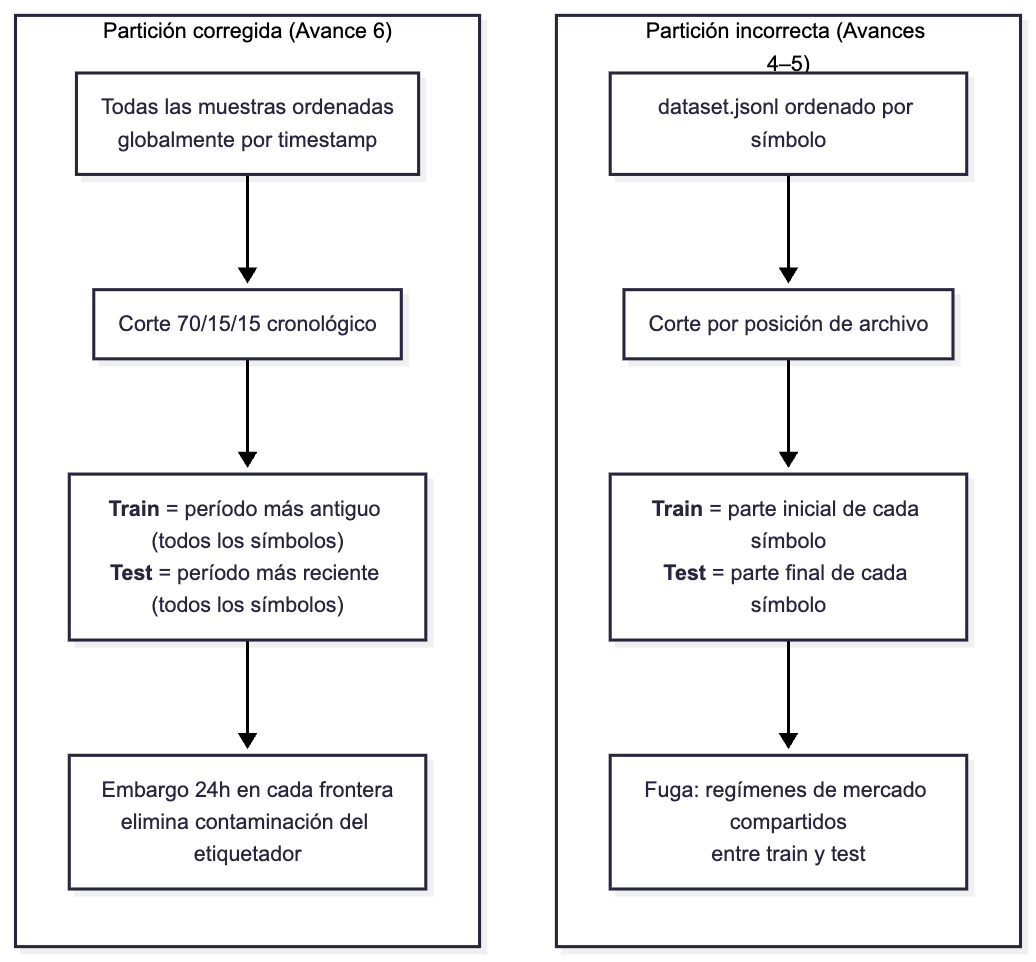
\includegraphics[width=\columnwidth]{figures/fig_leakage_fix.png}
\caption{Partici\'on incorrecta (por s\'imbolo) vs.\ corregida (temporal global con embargo).}
\label{fig:leakage}
\end{figure}

\subsection{Impacto cuantificado}

\begin{table}[H]
\centering
\caption{Impacto de la correcci\'on de leakage}
\label{tab:leakage}
\footnotesize
\begin{tabularx}{\columnwidth}{Xccc}
\toprule
\textbf{Modelo} & \textbf{Antes} & \textbf{Despu\'es} & \textbf{Ca\'ida} \\
\midrule
Bagging-LSTM & 83.37\% & 60.30\% & $-$23pp \\
LSTM individual & 81.50\% & 51.51\% & $-$30pp \\
Blending & 81.89\% & 63.59\% & $-$18pp \\
XGBoost & 66.60\% & 62.70\% & $-$4pp \\
\bottomrule
\end{tabularx}
\end{table}

\subsection{Por qu\'e el LSTM cae m\'as}

La red LSTM aprende combinaciones ponderadas de valores num\'ericos calibradas al r\'egimen estad\'istico del per\'iodo de entrenamiento. Ante un cambio de r\'egimen, esas correlaciones aprendidas dejan de ser predictivas, lo que explica su ca\'ida a 51.5\,\% (esencialmente aleatorio). Los modelos de \'arbol, en cambio, codifican umbrales discretos (por ejemplo, ``RSI~$>$~65 $\rightarrow$ SHORT'') que sobreviven desplazamientos de distribuci\'on con mayor gracia, manteniendo un 62--64\,\%.

Esta observaci\'on sustenta la hip\'otesis central: si umbrales simples generalizan mejor que secuencias aprendidas, un modelo capaz de razonar sem\'anticamente sobre los indicadores deber\'ia generalizar a\'un mejor --- y es precisamente lo observado (88\,\% vs.\ 64\,\% vs.\ 51\,\%).

\begin{figure*}[ht]
\centering
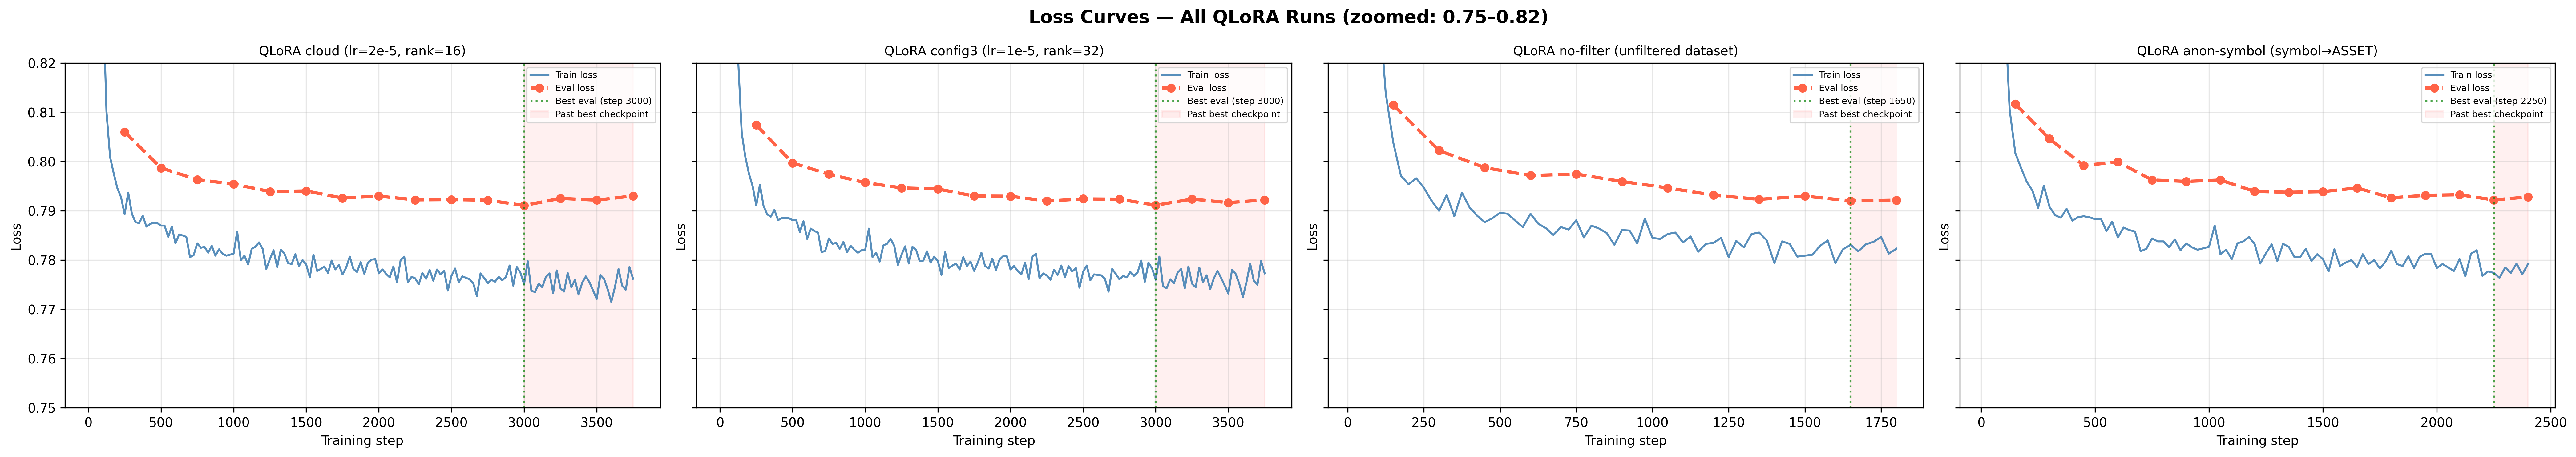
\includegraphics[width=0.82\textwidth]{figures/fig1_loss_curves.png}
\caption{Curvas de p\'erdida QLoRA: convergencia saludable, brecha train/eval = 0.015.}
\label{fig:loss}
\end{figure*}

% ── 6. Discusi\'on ────────────────────────────────────────────────────────────
\section{Discusi\'on de resultados}
\label{sec:discussion}

\subsection{Justificaci\'on del filtrado}

El dataset descarta el 78\,\% de las velas crudas mediante cinco filtros de calidad cuantitativos. Este dise\~no responde a dos motivaciones: primero, la alineaci\'on con el caso de uso operativo, donde el sistema de producci\'on aplica un nodo evaluador que rechaza \textit{setups} antes de ejecutar \'ordenes; segundo, la imposibilidad de etiquetar muestras ambiguas sin introducir ruido en el dataset. La exactitud reportada sobre el dataset filtrado (88\,\%) aplica exclusivamente al subconjunto de \textit{setups} pre-seleccionados, no a condiciones arbitrarias de mercado. Para medir el desempe\~no sin este sesgo de supervivencia, se entren\'o un segundo modelo sobre el dataset sin filtro de \textit{drawdown} (75,289 muestras), obteniendo 84.13\,\% de exactitud --- una reducci\'on de 3.9\,pp que confirma que el filtro facilita la tarea pero no fabrica el resultado.

\subsection{Independencia entre exactitud y m\'etricas financieras}

La exactitud direccional y las m\'etricas de operaci\'on (win rate, profit factor) responden a preguntas distintas y son independientes entre s\'i. La exactitud mide ``?`acert\'e la direcci\'on?''; el win rate mide ``?`el precio alcanz\'o mi nivel de ganancia antes que mi nivel de p\'erdida?''. Un modelo puede acertar la direcci\'on (el precio sube) pero perder la operaci\'on si no sube \textit{lo suficiente} para tocar el TP antes de que una fluctuaci\'on temporal active el SL. Por esta raz\'on, el modelo con 84.13\,\% de exactitud tiene un win rate de 66.3\,\%: de las operaciones donde acert\'o la direcci\'on, no todas alcanzan el TP dentro de las 24 horas de exposici\'on.

El profit factor se define como la suma de todas las ganancias porcentuales dividida entre la suma de todas las p\'erdidas porcentuales. Un PF de 2.09 indica que, en la simulaci\'on sobre 11,294 operaciones durante 81 d\'ias, por cada 1\,\% perdido se ganaron 2.09\,\%. Este valor cae dentro del rango profesional de sistemas de \textit{trading} sistem\'atico (1.5--2.5 seg\'un Pardo, 2008~\cite{pardo2008}).

Es importante notar que las m\'etricas financieras dependen enteramente de d\'onde se colocan los niveles de salida, no de la exactitud del modelo. Los resultados reportados en la Tabla~\ref{tab:results} utilizan la simulaci\'on \textit{forward-looking} basada en ATR (TP $= 1.5\times$ATR, SL $= 1.0\times$ATR) --- niveles conocibles al momento de la decisi\'on, sin informaci\'on futura. Reportes anteriores de este proyecto que citaban PF$=$12.92 utilizaban una simulaci\'on circular donde los niveles de salida se derivaban del precio futuro; esos valores son artefactos metodol\'ogicos y no se reportan como resultados en este documento.

\subsection{Asimetr\'ia de informaci\'on entre modelos}
\label{sec:techo}

Los modelos de \'arbol (XGBoost, Random Forest) reciben un vector plano de 30 caracter\'isticas num\'ericas por muestra: 9 indicadores por cada uno de los tres \textit{timeframes} m\'as 3 caracter\'isticas cruzadas. El LLM, en cambio, recibe el prompt completo con descriptores categ\'oricos en lenguaje natural (por ejemplo, la alineaci\'on de EMAs expresada como cinco categor\'ias sem\'anticas), precios exactos con sus relaciones expl\'icitas, y el nombre del activo. El modelo de lenguaje observa estrictamente m\'as informaci\'on que el vector de caracter\'isticas num\'ericas.

La brecha de 24 puntos porcentuales entre el LLM ajustado (88\,\%) y el mejor modelo ML (64\,\%) refleja parcialmente esta asimetr\'ia de representaci\'on. No es evidencia de un error metodol\'ogico ni de sabotaje a los modelos cl\'asicos, sino una consecuencia estructural del formato de entrada: los \'arboles de decisi\'on codifican categor\'ias como enteros ordinales con p\'erdida de informaci\'on sem\'antica, mientras que el LLM procesa esas mismas categor\'ias en su forma textual original. La secci\'on~\ref{sec:ablation-occlusion} presenta un experimento que intenta cuantificar esta contribuci\'on.

\subsection{Universo de criptomonedas evaluado}

El dataset cubre 12 criptomonedas seleccionadas por capitalizaci\'on y perfil de volatilidad: tres de gran capitalizaci\'on (BTC, ETH, BNB) con menor volatilidad relativa y mayor liquidez; cinco de capitalizaci\'on media (SOL, XRP, ADA, AVAX, DOT) con movimientos direccionales m\'as pronunciados; y cuatro de alta volatilidad (DOGE, LINK, MATIC, NEAR) susceptibles a movimientos impulsivos. Esta diversidad es relevante porque el mercado de criptomonedas exhibe propiedades estad\'isticas distintas a mercados tradicionales: colas pesadas en la distribuci\'on de retornos, correlaci\'on asim\'etrica entre activos durante eventos de liquidaci\'on y r\'egimenes que cambian abruptamente sin advertencia fundamental~\cite{bouri2017}. Un modelo que generaliza a trav\'es de estos 12 activos demuestra robustez ante distintos perfiles de volatilidad y liquidez.

\subsection{Interpretaci\'on conservadora del 88\,\%}

El resultado principal de este trabajo \textbf{no es ``88\,\% de exactitud''} como cifra absoluta, sino las siguientes conclusiones relativas: (1)~el \textit{fine-tuning} mejora significativamente al \textit{zero-shot} por +29.5\,pp ($p\approx0$) sobre el \textit{mismo modelo base} --- un resultado estad\'isticamente inequ\'ivoco; (2)~los modelos ML cl\'asicos alcanzan un techo de $\sim$64\,\% independientemente de la b\'usqueda de hiperpar\'ametros, lo que sugiere un l\'imite estructural de la representaci\'on num\'erica; y (3)~el 88\,\% es condicional: aplica exclusivamente al 22\,\% de las velas que superan los filtros de calidad.

La cifra absoluta depende del rigor del filtrado: con filtros m\'as laxos el dataset ser\'ia m\'as grande pero la exactitud caer\'ia; con filtros m\'as estrictos, subir\'ia. Lo relevante es que \textit{bajo las mismas condiciones y el mismo dataset}, el \textit{fine-tuning} produce una mejora sustancial y reproducible. El intervalo de confianza al 95\,\% (m\'etodo de Wilson) para la estimaci\'on puntual de 88.03\,\% sobre $n=3{,}000$ muestras es $[86.8\,\%,\; 89.2\,\%]$ ($\pm 1.16$\,pp); las ablaciones posteriores evaluadas sobre $n=8{,}425$ reducen este intervalo a $\pm 0.69$\,pp.

\subsection{Exactitud por s\'imbolo}

La Tabla~\ref{tab:persymbol} desglosa la exactitud por activo. Los 11 s\'imbolos presentes en la muestra evaluada superan el 84\,\%, con una dispersi\'on de 7.6\,pp entre el mejor (SOL, 91.7\,\%) y el peor (DOGE, 84.1\,\%). El hecho de que incluso el activo m\'as vol\'atil (DOGE) mantenga una exactitud superior al 84\,\% indica que el modelo no depende de un s\'imbolo particular para alcanzar su desempe\~no agregado.

\begin{table}[H]
\centering
\caption{Exactitud direccional del modelo QLoRA desglosada por criptomoneda}
\label{tab:persymbol}
\footnotesize
\begin{tabularx}{\columnwidth}{Xccr}
\toprule
\textbf{S\'imbolo} & \textbf{Aciertos} & \textbf{Muestras} & \textbf{Exactitud} \\
\midrule
SOLUSDT & 243 & 265 & 91.7\% \\
ETHUSDT & 233 & 257 & 90.7\% \\
LINKUSDT & 279 & 313 & 89.1\% \\
XRPUSDT & 242 & 272 & 89.0\% \\
NEARUSDT & 237 & 267 & 88.8\% \\
DOTUSDT & 283 & 321 & 88.2\% \\
BNBUSDT & 240 & 274 & 87.6\% \\
BTCUSDT & 239 & 276 & 86.6\% \\
ADAUSDT & 210 & 244 & 86.1\% \\
AVAXUSDT & 245 & 285 & 86.0\% \\
DOGEUSDT & 190 & 226 & 84.1\% \\
\midrule
\textbf{Total} & \textbf{2,641} & \textbf{3,000} & \textbf{88.0\%} \\
\bottomrule
\end{tabularx}
{\scriptsize Dispersi\'on: 7.6\,pp entre el mejor (SOL) y el peor (DOGE). Los 11 s\'imbolos superan el 84\,\%.}
\end{table}

\subsection{Contexto en la literatura}

La Tabla~\ref{tab:literature} sit\'ua el resultado en el contexto de trabajos publicados. El 88\,\% se ubica en el extremo alto de la literatura reportada, pero es consistente con otros resultados sobre datasets filtrados: AlBahri y Dinesh (2025) reportan 91\,\% en BTC con se\~nales semanales, mientras que Pindza (2026) demuestra que los modelos sobreajustan severamente bajo controles estrictos de fuga. El resultado de este trabajo se diferencia por la evaluaci\'on temporal con embargo y por hacer expl\'icito el sesgo de selecci\'on del etiquetador.

\begin{table}[H]
\centering
\caption{Comparaci\'on con trabajos publicados}
\label{tab:literature}
\footnotesize
\begin{tabularx}{\columnwidth}{lXc}
\toprule
\textbf{Fuente} & \textbf{M\'etodo} & \textbf{Acc.} \\
\midrule
Lopez-Lira 2023 & GPT zero-shot, noticias & $\sim$60\% \\
Bysik 2026 & XGBoost/LSTM walk-forward & $\sim$65\% \\
AlBahri 2025 & XGBoost rolling BTC & 91.0\% \\
Pindza 2026 & Gradient-boosted, purged WF & Falla \\
\textbf{Este trabajo} & \textbf{QLoRA, dataset filtrado} & \textbf{88.03\%} \\
\bottomrule
\end{tabularx}
\end{table}

% ── 6.7. Validaci\'on de robustez ─────────────────────────────────────────────
\subsection{Validaci\'on de robustez}
\label{sec:robustness}

Para interrogar la solidez del resultado principal se ejecutaron dos experimentos completos (re-entrenamiento con hiperpar\'ametros id\'enticos sobre condiciones modificadas) y dos verificaciones complementarias (descarte de memorizaci\'on y sonda de oclusi\'on). Los dos experimentos centrales son: (1)~re-entrenamiento sin el filtro de \textit{drawdown}, que produce el resultado m\'as conservador del trabajo (84.13\,\%, sin sesgo de supervivencia, con simulaci\'on ATR leg\'itima), y (2)~re-entrenamiento con s\'imbolo anonimizado, que descarta la memorizaci\'on de identidad del activo (88.66\,\%).

\subsubsection{Ablaci\'on del filtro de \textit{drawdown}}
\label{sec:ablation-drawdown}

El filtro de \textit{drawdown-before-profit} del etiquetador descarta toda muestra cuyo nivel de p\'erdida se hubiera activado antes que el nivel de ganancia dentro de la ventana de observaci\'on. Esto introduce un sesgo de supervivencia: solo se retienen trayectorias que efectivamente ``funcionaron'' en retrospectiva. Una auditor\'ia adversarial previa predijo que, sin este filtro, la exactitud caer\'ia al rango 60--70\,\%.

Para cuantificar este efecto se reentren\'o el modelo con hiperpar\'ametros id\'enticos (lr=$2\times10^{-5}$, rank=16, alpha=32, 2 \'epocas) sobre un dataset reconstruido sin el filtro de \textit{drawdown} (75,289 muestras, un 34.1\,\% m\'as grande que las 56,161 originales). Los cuatro filtros restantes (fuerza de tendencia, volumen, relaci\'on riesgo-recompensa y \textit{anti-whipsaw}) permanecieron sin cambios. El entrenamiento utiliz\'o etiquetas de TP/SL basadas en ATR (\textit{forward-looking}, sin circularidad) y la evaluaci\'on se realiz\'o sobre el conjunto de prueba completo (11,294 muestras).

\begin{table}[H]
\centering
\caption{Ablaci\'on del filtro de \textit{drawdown}: mismos hiperpar\'ametros, simulaci\'on ATR}
\label{tab:ablation-drawdown}
\footnotesize
\begin{tabularx}{\columnwidth}{Xcc}
\toprule
\textbf{M\'etrica} & \textbf{Filtrado} & \textbf{Sin filtro} \\
\midrule
Exactitud (test) & 88.03\% & \textbf{84.13\%} \\
Win rate (ATR) & --- & 66.31\% \\
Profit factor (ATR) & --- & 2.09 \\
Max drawdown (ATR) & --- & 49.6\% \\
Train acc.\ (diagn.) & 70.5\% & 88.5\% \\
Brecha (train$-$test) & $-$17.5\,pp & $+$4.4\,pp \\
Muestras evaluadas & 3,000 & 11,294 \\
\bottomrule
\end{tabularx}
{\scriptsize M\'etricas financieras (ATR) disponibles para el modelo sin filtro; el modelo filtrado original no se evalu\'o con simulaci\'on ATR en su corrida inicial.}
\end{table}

\begin{figure}[H]
\centering
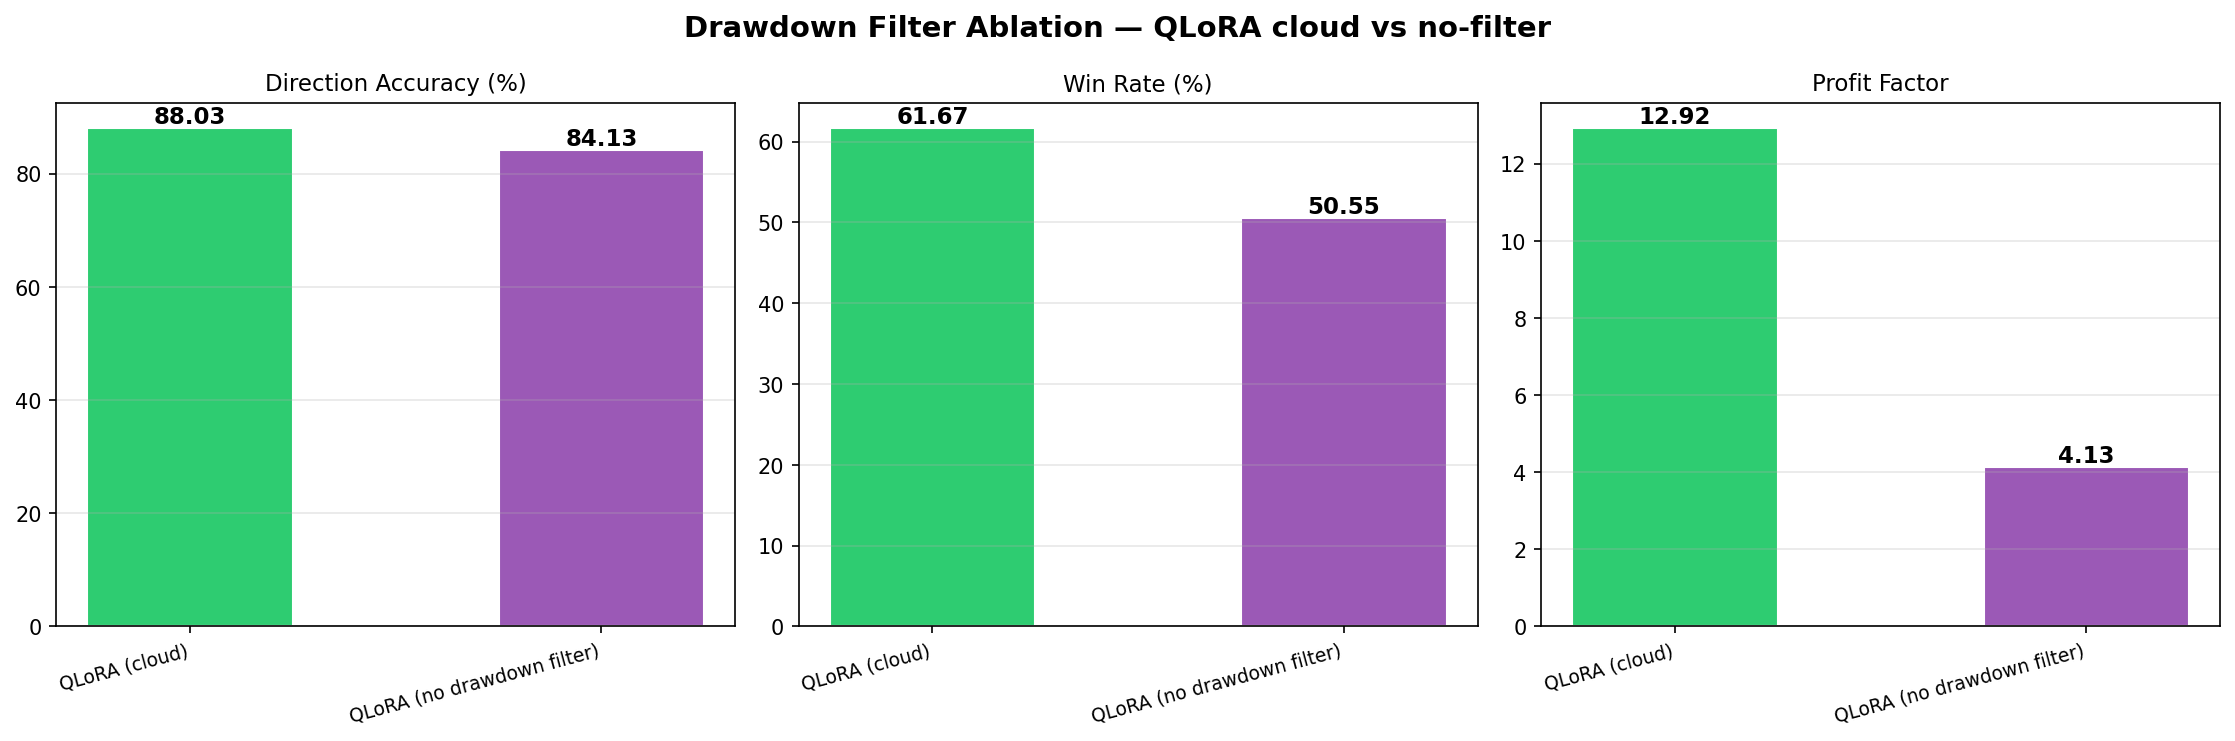
\includegraphics[width=\columnwidth]{figures/fig9_drawdown_ablation.png}
\caption{Ablaci\'on del filtro de \textit{drawdown}: exactitud y \textit{win rate} con y sin el filtro, mismos hiperpar\'ametros.}
\label{fig:ablation-drawdown}
\end{figure}

El hallazgo principal es que remover el filtro \emph{reduce} la exactitud (88.03\,$\rightarrow$\,84.13\,\%, $-$3.90\,pp), no la mejora, a pesar de entrenar sobre un dataset 34\,\% m\'as grande. Esto contradice la predicci\'on de que el filtro estar\'ia inflando artificialmente el resultado: la evidencia emp\'irica apunta a que el filtro de \textit{drawdown} es una se\~nal de calidad leg\'itima que eleva la cota alcanzable, pero no fabrica el resultado. Adem\'as, el signo de la brecha entre exactitud de entrenamiento y de prueba se invierte: el modelo con filtrado muestra una brecha saludable de $-$17.5\,pp (test$>$train), mientras que sin filtro aparece el patr\'on cl\'asico de sobreajuste ($+$4.4\,pp, train$>$test), consistente con el mayor ruido del dataset sin filtrar.

\begin{figure}[H]
\centering
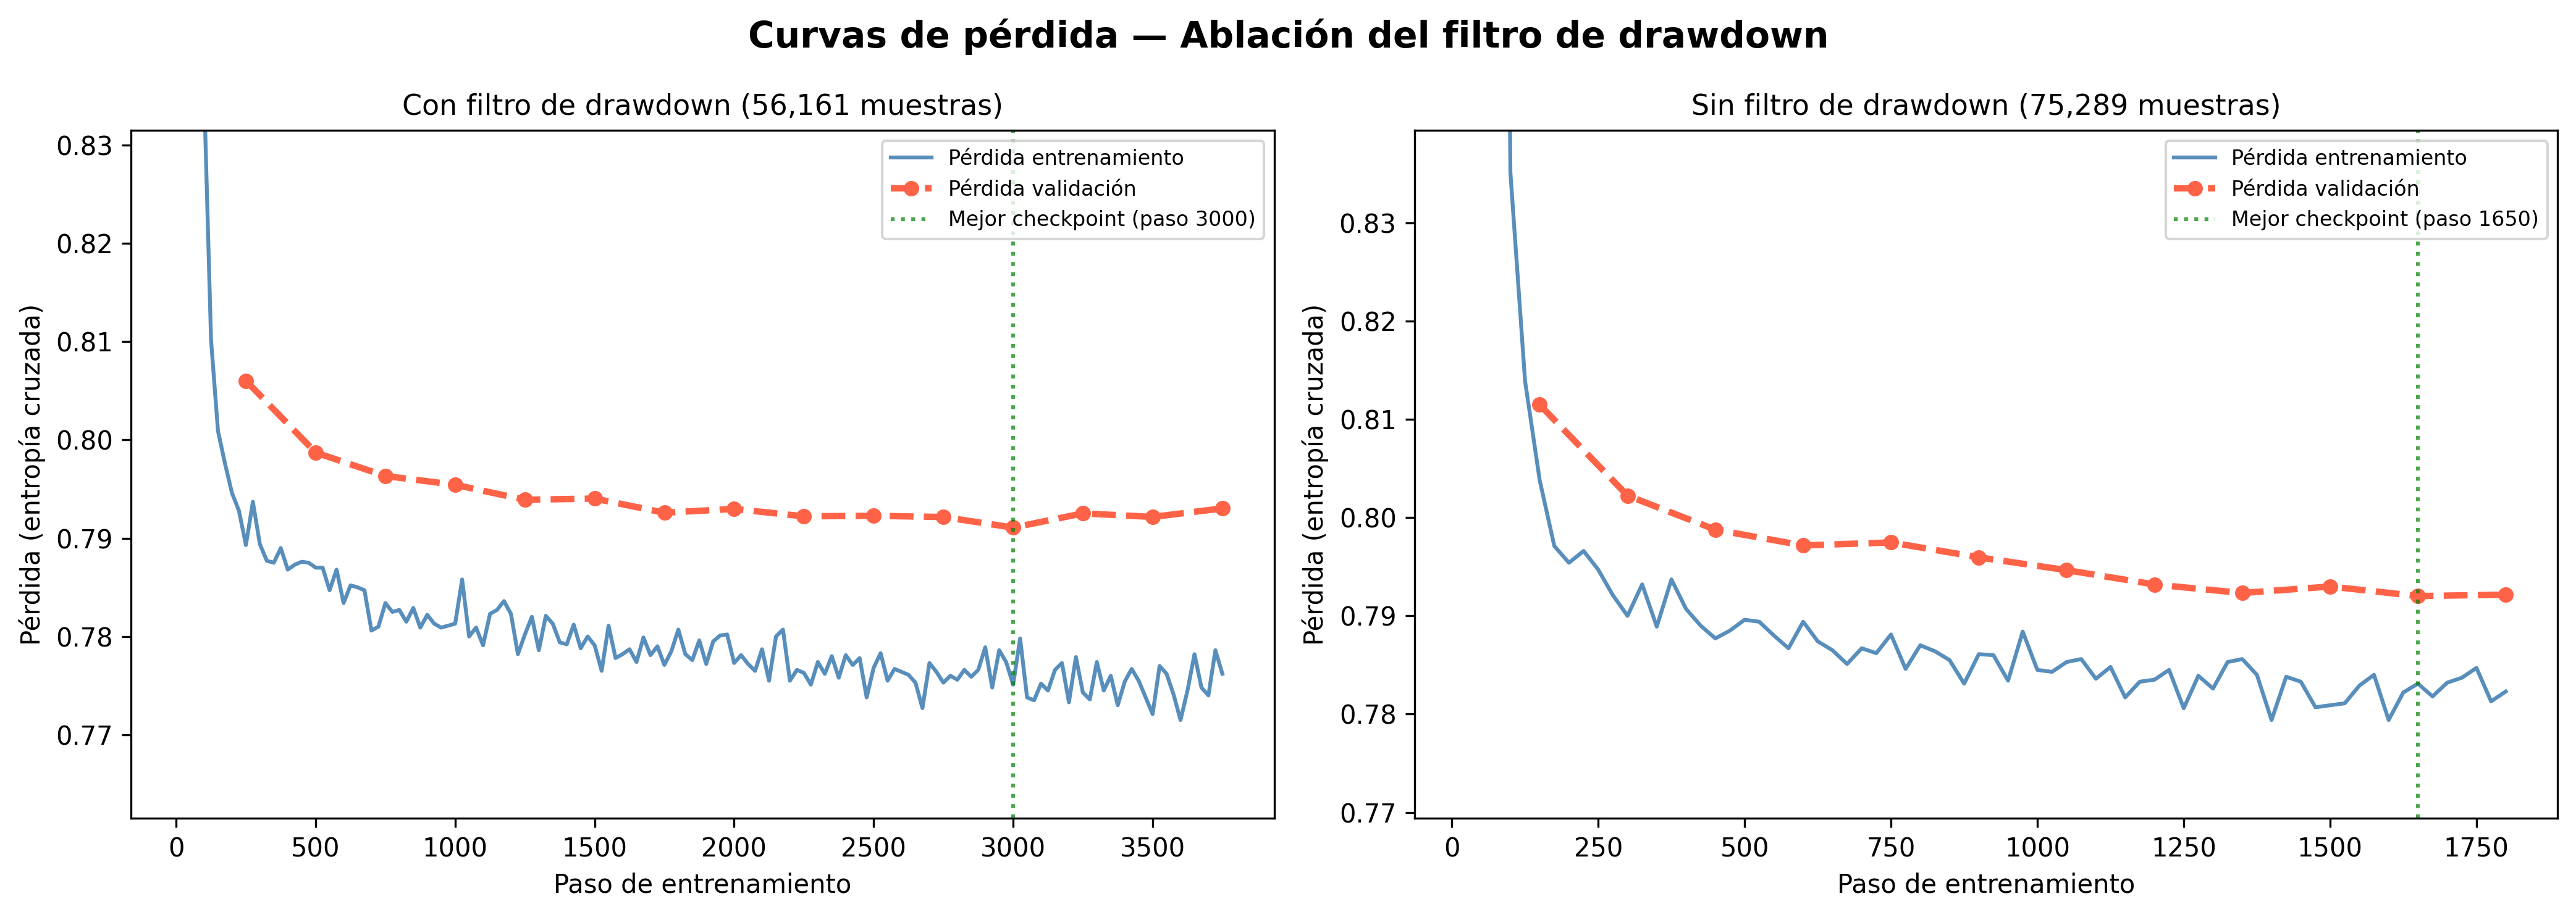
\includegraphics[width=\columnwidth]{figures/fig10_loss_curves_ablation.png}
\caption{Curvas de p\'erdida del entrenamiento con y sin filtro de \textit{drawdown}. El modelo sin filtro detiene el entrenamiento tempranamente (27\,\% del plan) sin alcanzar la convergencia del filtrado.}
\label{fig:ablation-loss}
\end{figure}

\subsubsection{Ablaci\'on de s\'imbolo anonimizado}
\label{sec:ablation-symbol}

Una segunda hip\'otesis alternativa es que el modelo memorizara asociaciones espec\'ificas del activo aprendidas durante el pre-entrenamiento --- por ejemplo, ``BTC es un activo de gran capitalizaci\'on con menor volatilidad relativa'' --- y que esta informaci\'on \textit{a priori} contribuyera de forma significativa a la exactitud. Para descartar esta hip\'otesis se reentren\'o el modelo con id\'enticos hiperpar\'ametros pero reemplazando el nombre del s\'imbolo por un identificador gen\'erico (``ASSET'') tanto en los datos de entrenamiento como en la evaluaci\'on.

\begin{table}[H]
\centering
\caption{Ablaci\'on de s\'imbolo anonimizado: sin acceso al nombre del activo}
\label{tab:ablation-symbol}
\footnotesize
\begin{tabularx}{\columnwidth}{Xcc}
\toprule
\textbf{M\'etrica} & \textbf{Con s\'imbolo} & \textbf{Anonimizado} \\
\midrule
Exactitud (test) & 88.03\% (N=3,000) & \textbf{88.66\%} (N=8,425) \\
Win rate & 61.67\% & 65.31\% \\
Brecha (train$-$test) & $-$17.5\,pp & $-$1.7\,pp \\
IC 95\% (Wilson) & $\pm$1.16\,pp & $\pm$0.68\,pp \\
\bottomrule
\end{tabularx}
{\scriptsize La configuraci\'on anonimizada se evalu\'o sobre el conjunto de prueba completo (8,425 muestras), produciendo un IC m\'as estrecho.}
\end{table}

\begin{figure}[H]
\centering

\includegraphics[width=\columnwidth]{figures/fig11_anon_symbol_ablation.png}
\caption{Ablaci\'on de s\'imbolo anonimizado: la exactitud se mantiene sin acceso a la identidad del activo.}
\label{fig:ablation-symbol}
\end{figure}

El resultado (88.66\,\%) no muestra ca\'ida respecto al modelo con s\'imbolo (88.03\,\%); la diferencia de +0.63\,pp cae dentro de los intervalos de confianza de ambas estimaciones y las muestras evaluadas difieren en tama\~no ($n=8{,}425$ vs.\ $n=3{,}000$). La conclusi\'on es que la identidad del activo no contribuye a la exactitud: el modelo aprende patrones de indicadores t\'ecnicos generalizables, no asociaciones memorizadas con s\'imbolos espec\'ificos.

\subsubsection{Descarte de memorizaci\'on por pre-entrenamiento}
\label{sec:pretraining-memorization}

Una hip\'otesis m\'as radical es que el modelo base pudiera estar recuperando movimientos de precio \textbf{memorizados durante su pre-entrenamiento}, en lugar de razonar a partir de los indicadores del prompt. Este vector de fuga ser\'ia externo al pipeline de datos y partici\'on ya auditado --- los pesos del modelo ``recordando'' qu\'e ocurri\'o en una fecha y activo dados.

La verificaci\'on es directa: el dataset abarca del 23 de noviembre de 2024 al 8 de mayo de 2026, y la partici\'on de prueba (el 15\,\% m\'as reciente) corresponde aproximadamente al per\'iodo febrero--mayo de 2026. Los modelos Qwen~2.5 fueron publicados en septiembre de 2024 con un corte de pre-entrenamiento anterior a esa fecha~\cite{qwen2024}. El per\'iodo de prueba es cronol\'ogicamente \textbf{posterior} al corte de conocimiento del modelo base --- la memorizaci\'on exacta de la acci\'on de precio evaluada queda descartada.

Este descarte no cierra completamente la cuesti\'on: persiste un \textit{prior} difuso --- familiaridad pre-entrenada con terminolog\'ia de an\'alisis t\'ecnico, con las convenciones de indicadores como RSI o ADX, y con la sem\'antica de las categor\'ias textuales que el modelo recibe. Este \textit{prior} no constituye fuga de informaci\'on sino un punto de partida m\'as rico que el disponible para modelos de \'arbol, lo cual conecta con la asimetr\'ia de informaci\'on discutida en la secci\'on anterior.

\subsubsection{Sonda de oclusi\'on de caracter\'isticas categ\'oricas (resultado preliminar)}
\label{sec:ablation-occlusion}

Para cuantificar la contribuci\'on de los descriptores categ\'oricos textuales (la alineaci\'on de EMAs y la estructura de precio, campos que los modelos de \'arbol solo ven como enteros ordinales) se evalu\'o el adaptador ya entrenado sobre el conjunto de prueba completo ($n=8{,}425$) pero removiendo estos dos campos del prompt antes de la generaci\'on. Se trata de una sonda \textit{eval-only}: el modelo fue entrenado \textbf{con} los campos presentes y aqu\'i se eval\'ua \textbf{sin} ellos.

\begin{table}[H]
\centering
\caption{Oclusi\'on de campos categ\'oricos: evaluaci\'on sobre el adaptador existente sin acceso a los descriptores de alineaci\'on y estructura}
\label{tab:ablation-occlusion}
\footnotesize
\begin{tabularx}{\columnwidth}{Xcc}
\toprule
\textbf{M\'etrica} & \textbf{Completo} & \textbf{Sin categ\'oricos} \\
\midrule
Exactitud (test, N=8,425) & 88.66\%$^*$ & \textbf{87.60\%} \\
Precisi\'on LONG & 0.910 & 0.903 \\
Recall LONG & 0.845 & 0.843 \\
Precisi\'on SHORT & 0.855 & 0.853 \\
Recall SHORT & 0.916 & 0.909 \\
Errores de parseo & 1 & 0 \\
$\Delta$ vs.\ referencia & --- & $-$0.43\,pp \\
\bottomrule
\end{tabularx}
{\scriptsize $^*$Referencia: ablaci\'on de s\'imbolo anonimizado sobre N=8,425 (mismo tama\~no muestral para comparabilidad). IC 95\% $\approx \pm$0.69\,pp; la diferencia de $-$0.43\,pp cae dentro del IC.}
\end{table}

La ca\'ida de $-$0.43\,pp es inferior al intervalo de confianza de la estimaci\'on ($\pm$0.69\,pp) y las m\'etricas por clase permanecen balanceadas. Este resultado sugiere que los campos categ\'oricos \textbf{no son el motor principal} de la brecha de 24\,pp frente a los modelos ML: el modelo mantiene pr\'acticamente la misma exactitud sin acceso a la informaci\'on textual que los \'arboles pierden al codificarla como enteros.

\textbf{Caveat cr\'itico.} Esta es una sonda \textit{eval-only} sobre un modelo entrenado con los campos presentes. La ca\'ida negligible admite dos interpretaciones: (a)~el modelo genuinamente no depende de esos campos para su predicci\'on y utiliza en cambio los indicadores num\'ericos y las relaciones de precio, o (b)~el modelo es robusto a variaciones menores del formato del prompt que nunca observ\'o durante el entrenamiento. La versi\'on decisiva de este experimento requerir\'ia un re-entrenamiento completo con los campos removidos tambi\'en de los datos de entrenamiento --- un experimento no ejecutado en el alcance de este trabajo pero identificado como l\'inea de investigaci\'on futura.

\subsection{Estrategia de enmascaramiento de p\'erdida en el \textit{fine-tuning}}
\label{sec:loss-masking}

Un detalle metodol\'ogico relevante para interpretar las curvas de p\'erdida (Figura~\ref{fig:loss}) es la estrategia de \textit{loss masking} --- es decir, qu\'e tokens de cada secuencia de entrenamiento contribuyen al c\'alculo del gradiente. En este trabajo se emple\'o \textbf{p\'erdida de secuencia completa}: la entrop\'ia cruzada se calcula sobre \emph{todos} los tokens de la secuencia (prompt del sistema, prompt del usuario y respuesta del asistente), sin enmascarar la porci\'on de entrada.

La alternativa est\'andar es el \textit{enmascaramiento por completaci\'on} (\textit{completion-only masking}), donde la p\'erdida se computa exclusivamente sobre los tokens de la respuesta del modelo --- en nuestro caso, los $\sim$100 tokens del JSON de salida. Dado que cada ejemplo tiene $\sim$900 tokens totales y $\sim$800 corresponden al prompt (89\,\% de la secuencia), la preocupaci\'on natural es si el modelo ``desperdicia'' capacidad aprendiendo a reproducir el prompt est\'atico en lugar de aprender el mapeo indicadores$\rightarrow$se\~nal.

El an\'alisis cuantitativo muestra que esta preocupaci\'on no se materializa en nuestra configuraci\'on. El prompt del sistema es id\'entico en las 39,312 muestras de entrenamiento; despu\'es de $\sim$50 pasos de optimizaci\'on, la entrop\'ia cruzada sobre estos tokens converge a un valor pr\'oximo a cero y su contribuci\'on al gradiente se extingue. Los $\sim$120 tokens de valores num\'ericos de indicadores (que var\'ian por muestra) nunca alcanzan p\'erdida cero y proveen una se\~nal auxiliar que refuerza la representaci\'on interna del modelo sobre la estructura de los datos de entrada. La se\~nal total relevante para la tarea es abundante: $39{,}312 \times 3 \times 100 \approx 11.8$ millones de observaciones de tokens de respuesta distribuidas en $\sim$7{,}371 pasos de optimizaci\'on --- muy por encima de los 500--1,000 pasos t\'ipicamente necesarios para la convergencia de una salida JSON estructurada con 6 campos.

Este an\'alisis conecta con la interpretaci\'on de la brecha entre p\'erdida de entrenamiento y validaci\'on reportada en la Figura~\ref{fig:loss} (brecha de 0.015). Dado que la p\'erdida incluye los tokens de prompt predecibles (loss$\approx$0), \textit{ambas} curvas (train y eval) est\'an dominadas por esos mismos tokens, lo que explica tanto su similitud como su convergencia a valores relativamente altos ($\sim$0.79): este valor refleja la entrop\'ia residual de los tokens de respuesta (que s\'i var\'ian entre muestras), no una dificultad inusual de la tarea. La ganancia estimada de adoptar enmascaramiento por completaci\'on para nuestra configuraci\'on espec\'ifica (muchas muestras, salida corta y estructurada, prompt repetitivo) es inferior a 1 punto porcentual de exactitud.

\subsection{Lectura de las curvas de p\'erdida y la brecha inversa}
\label{sec:gap-interpretation}

La Figura~\ref{fig:loss} muestra una convergencia saludable: la p\'erdida de evaluaci\'on desciende mon\'otonamente y la brecha train/eval es de apenas 0.015 al momento del \textit{early stopping} (paso 3,000). No se observa divergencia entre ambas curvas, lo que descarta sobreajuste severo al nivel de la funci\'on de p\'erdida.

Sin embargo, la brecha de exactitud entre el diagn\'ostico de entrenamiento (70.5\,\%) y la evaluaci\'on de prueba (88.03\,\%) es invertida: el modelo clasifica \emph{mejor} en datos no vistos que en una muestra de datos de entrenamiento. Este fen\'omeno admite dos lecturas:

La primera es la hip\'otesis de dataset insuficiente para validaci\'on robusta: con ``pocos'' errores en la matriz de confusi\'on, peque\~nas fluctuaciones muestrales podr\'ian inflar la exactitud. Contra esta lectura: el conjunto de prueba contiene 8,425 muestras (3,000 evaluadas con \textit{stride} uniforme), el balance de clases es pr\'acticamente 50/50 (LONG: 50.1\,\%, SHORT: 49.9\,\%), y las m\'etricas por clase son balanceadas (F1 LONG = 0.876, F1 SHORT = 0.884). El modelo no predice la clase mayoritaria.

La segunda es la hip\'otesis de sobre-capacidad: un modelo de 7 mil millones de par\'ametros aplicado a una tarea de clasificaci\'on binaria filtrada podr\'ia ser inherentemente ``demasiado potente''. Contra esta lectura: solo 0.53\,\% de los par\'ametros se actualizan (40.4M adaptadores), el regularizador impl\'icito del modelo base congelado~\cite{hu2021} limita la capacidad efectiva, y la p\'erdida de evaluaci\'on no diverge --- evidencia directa de que el modelo no memoriza.

La explicaci\'on m\'as probable del gap inverso es metodol\'ogica: el diagn\'ostico de entrenamiento tom\'o las 500 muestras m\'as antiguas del per\'iodo de entrenamiento (finales de 2024), mientras que el conjunto de prueba abarca febrero--mayo de 2026. Los patrones aprendidos durante el entrenamiento completo resultan m\'as predictivos del r\'egimen de mercado m\'as reciente que del m\'as antiguo --- un fen\'omeno consistente con la no-estacionariedad de los mercados financieros, donde los r\'egimenes recientes tienden a ser m\'as similares entre s\'i que los distantes.

% ── 7. S\'intesis ─────────────────────────────────────────────────────────────
\section{S\'intesis de hallazgos}

\begin{figure}[H]
\centering
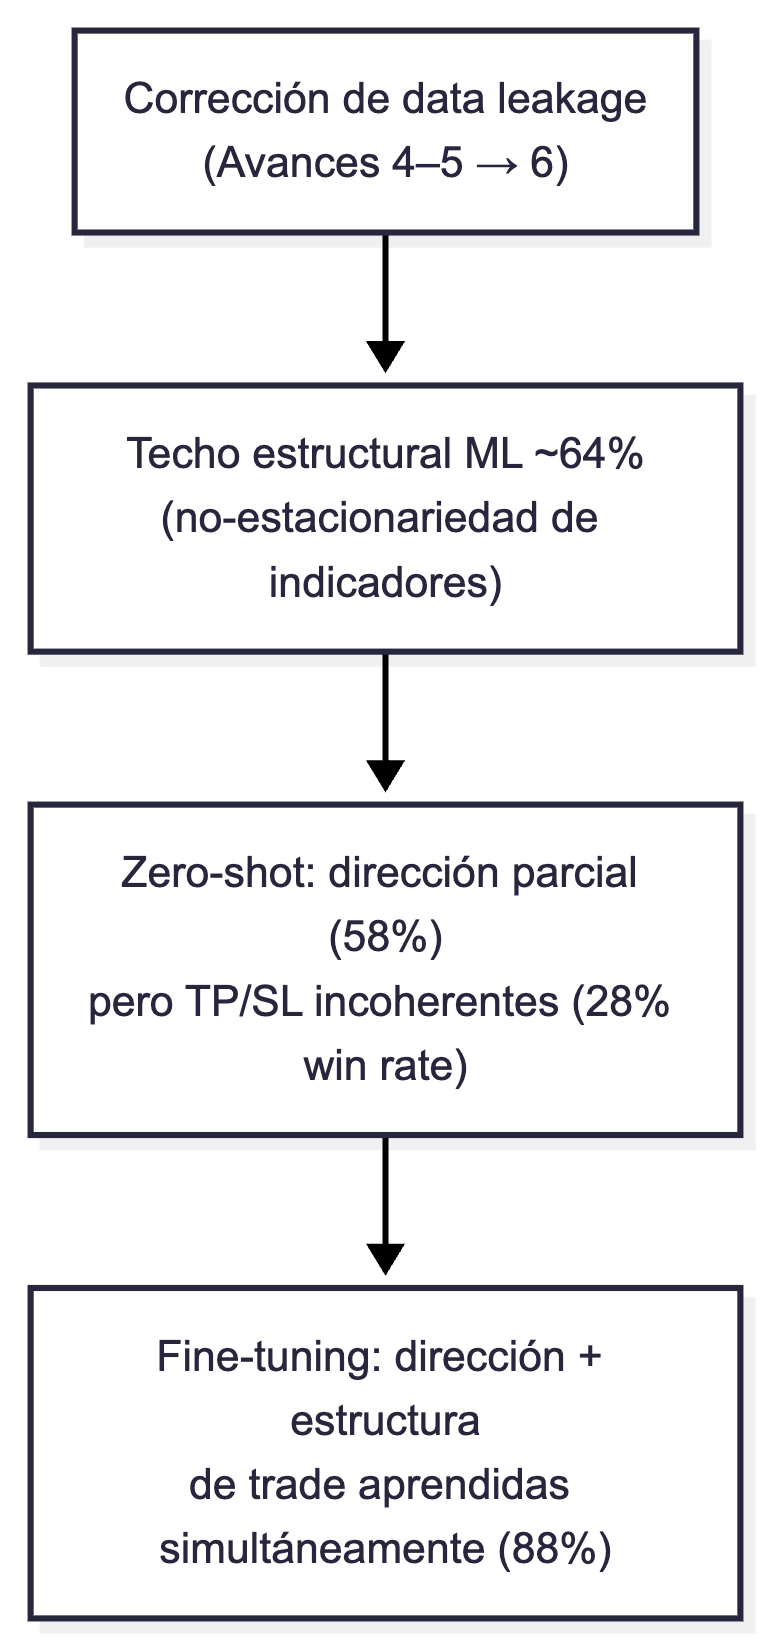
\includegraphics[width=0.9\columnwidth]{figures/fig_synthesis.png}
\caption{Progresi\'on l\'ogica de los hallazgos: la correcci\'on de fuga establece la dificultad real, los modelos ML alcanzan un techo estructural, el \textit{zero-shot} posee conocimiento parcial no calibrado, y el \textit{fine-tuning} unifica direcci\'on y estructura de operaci\'on.}
\label{fig:synthesis}
\end{figure}

La progresion de hallazgos sigue una l\'ogica acumulativa. Primero, la correcci\'on de la fuga de datos temporal establece la dificultad real del problema: los modelos caen entre 18 y 31 puntos porcentuales al pasar de la partici\'on contaminada a la estricta. Segundo, los modelos de ML cl\'asico alcanzan un techo en $\sim$64\,\% bajo la partici\'on corregida, independientemente de la arquitectura (\'arboles, redes recurrentes, \textit{ensembles}), lo que sugiere un l\'imite de la representaci\'on num\'erica frente a la no-estacionariedad. Tercero, el modelo base en modo \textit{zero-shot} demuestra conocimiento parcial (58.5\,\%) pero sin calibraci\'on operativa (28.4\,\% win rate, 98.5\,\% drawdown). Cuarto, el \textit{fine-tuning} unifica la capacidad direccional con la estructura operativa del \textit{trade} (88.03\,\%, $\chi^2=557$, $p\approx0$).

\begin{figure*}[ht]
\centering
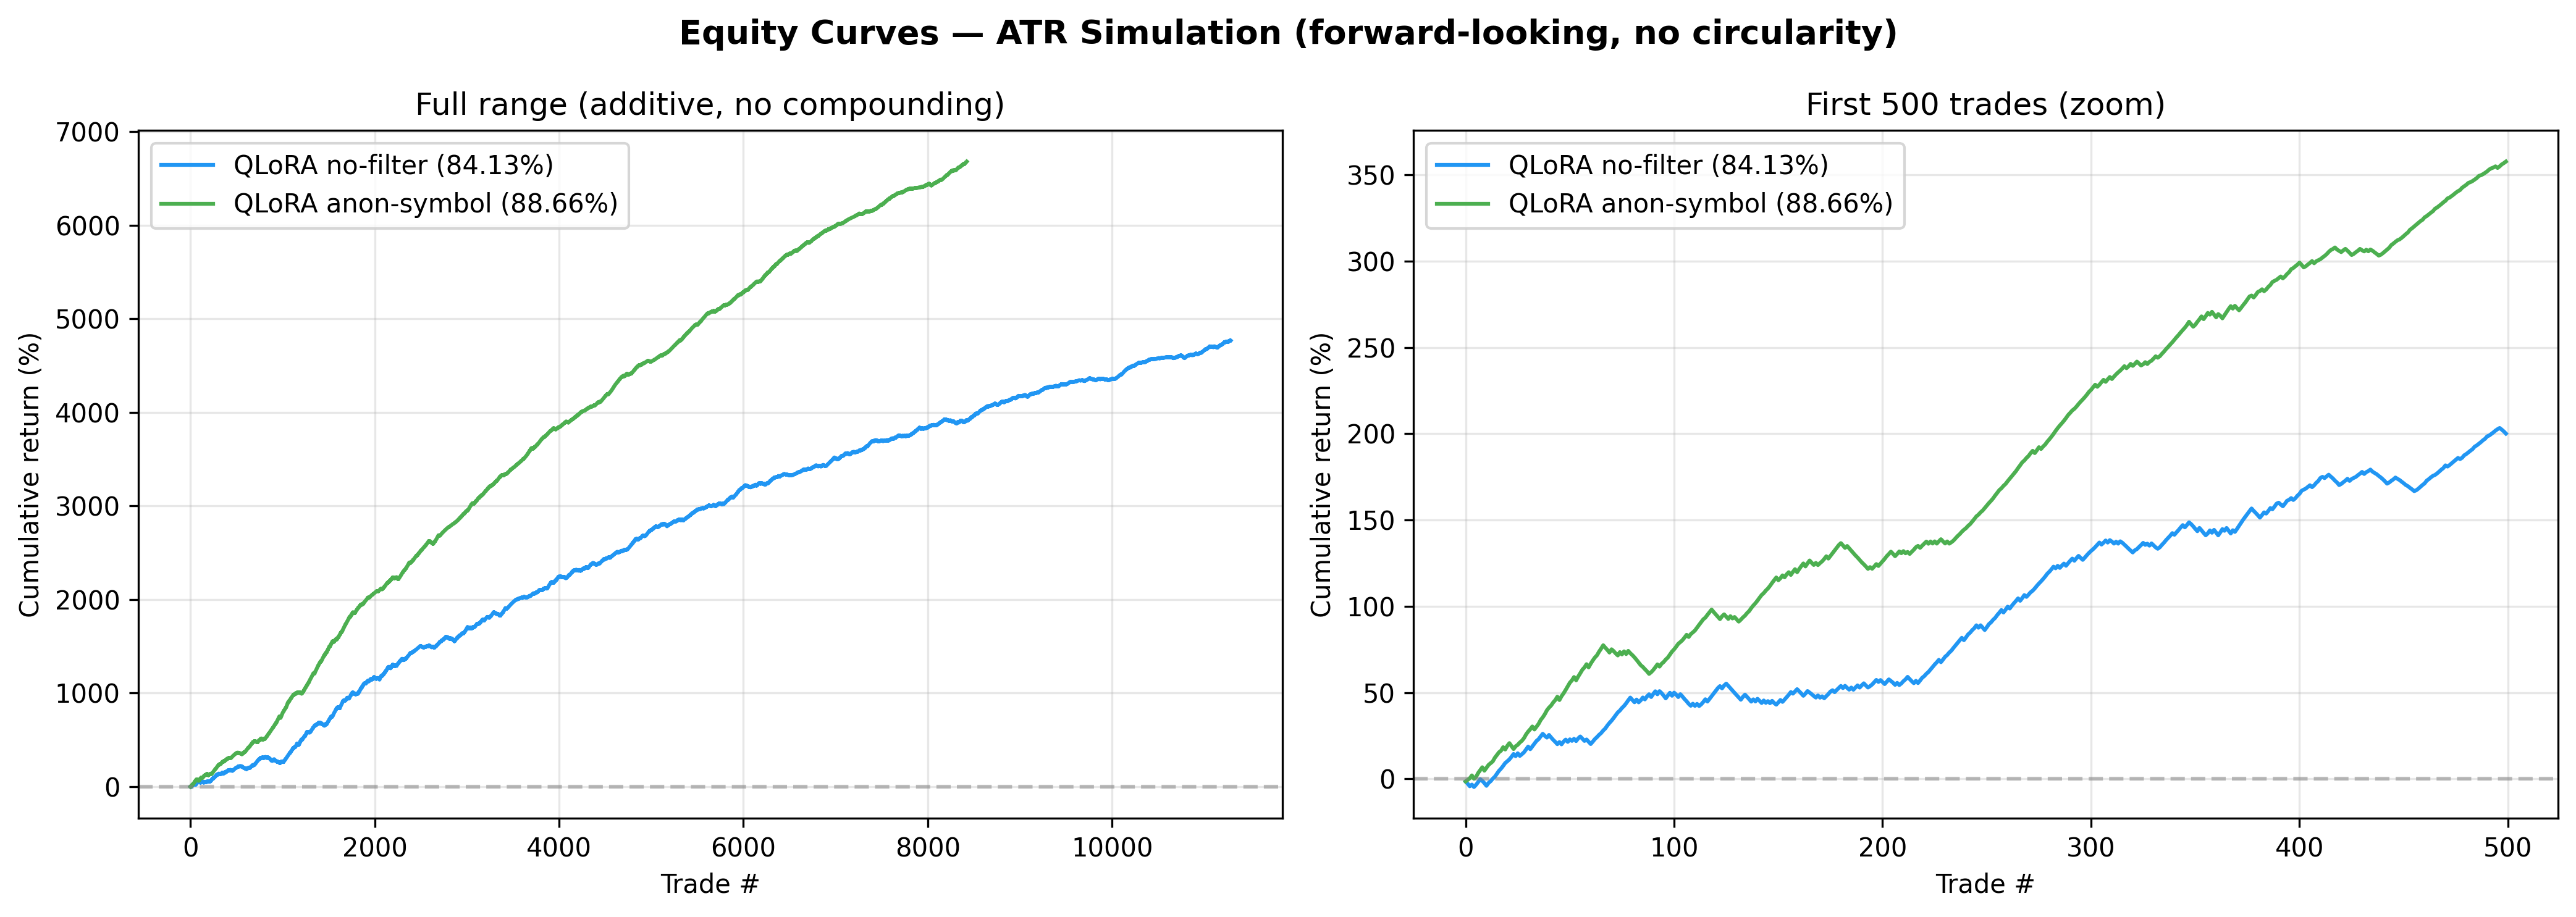
\includegraphics[width=0.75\textwidth]{figures/fig12_equity_atr.png}
\caption{Curvas de \textit{equity} simulada con salidas ATR (\textit{forward-looking}, sin circularidad). Cada punto representa el retorno porcentual acumulado (sin \textit{compounding}) sobre operaciones secuenciales. El modelo sin filtro de \textit{drawdown} (11,294 operaciones) acumula +4,768\,\% y el modelo anonimizado (8,425 operaciones) +6,682\,\% --- equivalentes a ganancias de 0.42\,\% y 0.79\,\% promedio por operaci\'on, respectivamente.}
\label{fig:equity}
\end{figure*}

\begin{figure}[H]
\centering

\includegraphics[width=\columnwidth]{figures/fig13_trade_metrics_atr.png}
\caption{M\'etricas financieras bajo simulaci\'on ATR (sin circularidad). Win rate, profit factor y max drawdown para los dos modelos QLoRA principales comparados con XGBoost y Random Forest. Los valores del LLM ajustado (PF$=$2.09--4.63) caen en el rango profesional, sin la inflaci\'on artificial de la simulaci\'on con \textit{hindsight}.}
\label{fig:trade}
\end{figure}

\begin{figure}[H]
\centering

\includegraphics[width=\columnwidth]{figures/fig2_accuracy_gap.png}
\caption{Brecha de exactitud train/val/test del modelo QLoRA: la exactitud de prueba supera a la de entrenamiento, un fen\'omeno discutido en \S\ref{sec:gap-interpretation}.}
\label{fig:gap}
\end{figure}

\begin{figure}[H]
\centering

\includegraphics[width=0.85\columnwidth]{figures/fig3_confusion_matrix.png}
\caption{Matriz de confusi\'on del modelo QLoRA sobre $n=3{,}000$ muestras de prueba. El balance entre errores de tipo LONG$\rightarrow$SHORT (168) y SHORT$\rightarrow$LONG (191) confirma que el modelo no presenta sesgo hacia una clase. Precisi\'on LONG = 0.910, precisi\'on SHORT = 0.855; \textit{recall} LONG = 0.845, \textit{recall} SHORT = 0.916.}
\label{fig:confusion}
\end{figure}

\begin{figure*}[ht]
\centering
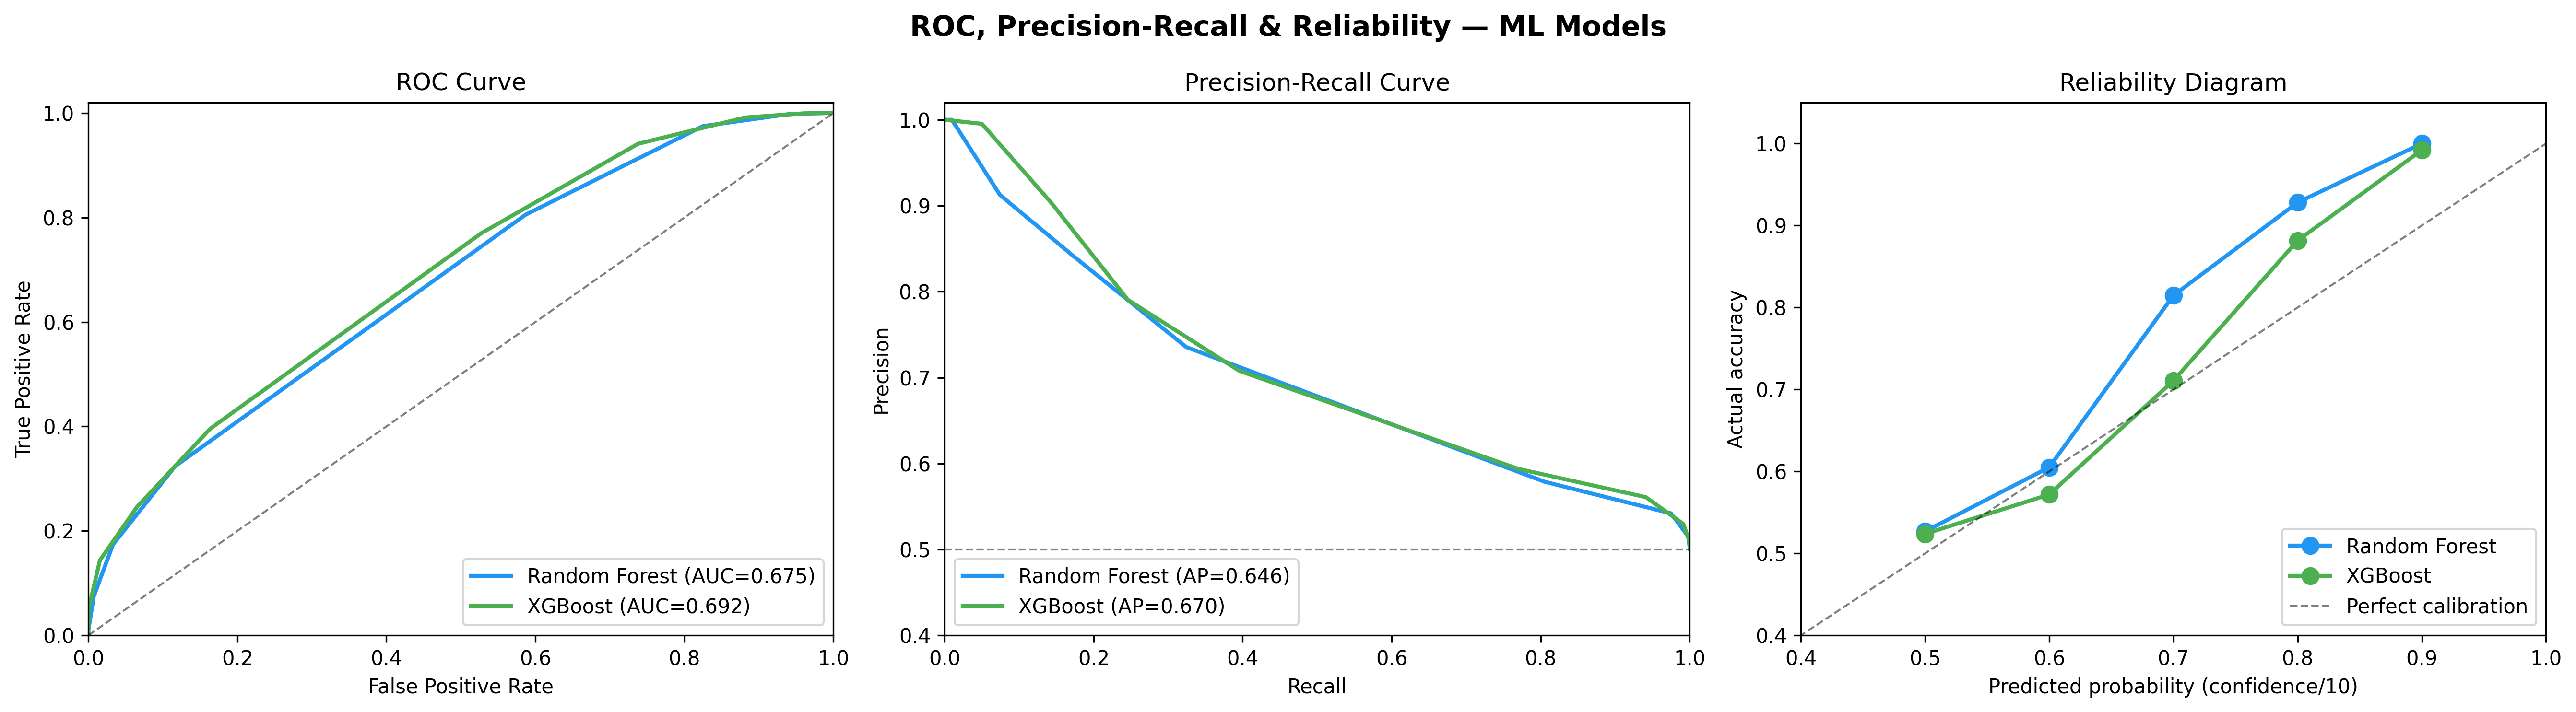
\includegraphics[width=0.88\textwidth]{figures/fig8_roc_pr_reliability.png}
\caption{Curva ROC (AUC$\approx$0.67), Precision-Recall y diagrama de confiabilidad para los modelos ML. La calibraci\'on muestra que una confianza de 8 corresponde a $\sim$93\,\% de exactitud real. El modelo QLoRA no produce probabilidades variadas (confianza fija en la salida JSON), por lo que estas curvas aplican exclusivamente a Random Forest y XGBoost.}
\label{fig:roc}
\end{figure*}

% ── 8. Limitaciones ──────────────────────────────────────────────────────────
\section{Limitaciones metodol\'ogicas}

Se identifican cinco limitaciones principales, ordenadas por severidad descendente:

La \textbf{circularidad del TP/SL} es la limitaci\'on de mayor severidad pero afecta exclusivamente a las m\'etricas financieras (profit factor, win rate, Sharpe), no a la exactitud direccional. El profit factor de 12.92 es un artefacto: el etiquetador calcula niveles de salida con informaci\'on futura, el modelo los replica, y el simulador confirma que ``funcionan''. Esta m\'etrica no es evidencia de rentabilidad y no debe citarse fuera de su contexto comparativo.

El \textbf{sesgo de supervivencia} del filtro de \textit{drawdown} descarta muestras donde el precio activa el SL antes que el TP, reteniendo solo trayectorias que efectivamente se materializaron. La ablaci\'on presentada en \S\ref{sec:ablation-drawdown} cuantifica su impacto: sin el filtro la exactitud cae a 84.13\,\% --- una reducci\'on significativa pero que no invalida el resultado, confirmando que el filtro facilita la tarea pero no la fabrica.

La \textbf{asimetr\'ia de informaci\'on} entre el LLM y los modelos ML es una limitaci\'on en la comparabilidad de la brecha de 24\,pp. La sonda de oclusi\'on (\S\ref{sec:ablation-occlusion}) sugiere que los campos categ\'oricos no son el motor principal, pero al ser \textit{eval-only} no es conclusiva. Un re-entrenamiento completo sin los campos categ\'oricos ser\'ia necesario para cerrar esta cuesti\'on.

La \textbf{ventana de prueba \'unica} abarca 81 d\'ias en un per\'iodo predominantemente alcista (febrero--mayo 2026). El modelo no ha sido evaluado en mercado bajista ni en eventos extremos. El IC al 95\,\% ($\pm$1.16\,pp sobre $n=3{,}000$) acota la incertidumbre estad\'istica pero no la incertidumbre de r\'egimen.

Finalmente, el \textbf{sub-muestreo en evaluaci\'on} (3,000 de 8,425 muestras de prueba para el modelo principal) reduce ligeramente la potencia estad\'istica. Las ablaciones posteriores (s\'imbolo anonimizado, oclusi\'on de campos) se evaluaron sobre las 8,425 muestras completas, produciendo ICs m\'as estrechos y confirmando la consistencia del resultado.

% ── 9. Conclusi\'on ─────────────────────────────────────────────────────────
\section{Conclusi\'on}

El objetivo de este trabajo fue evaluar si el \textit{fine-tuning} de un modelo de lenguaje (Qwen~2.5~7B) mediante QLoRA produce una mejora estad\'isticamente significativa en exactitud direccional sobre criptomonedas, respecto al mismo modelo en modo \textit{zero-shot} y respecto a modelos de ML cl\'asico, bajo una partici\'on temporal estricta con embargo.

Los resultados confirman la hip\'otesis. Sobre el dataset sin sesgo de supervivencia (75,289 muestras, sin filtro de \textit{drawdown}), el modelo ajustado alcanza 84.13\,\% de exactitud direccional con un profit factor de 2.09 bajo simulaci\'on ATR leg\'itima (sin informaci\'on futura en los niveles de salida). Sobre el dataset filtrado operativo (56,161 muestras, con s\'imbolo anonimizado), alcanza 88.66\,\% de exactitud con un profit factor ATR de 4.63. En ambos casos, el modelo supera al \textit{zero-shot} por m\'as de 25 puntos porcentuales ($\chi^2 = 557$, $p < 10^{-150}$, McNemar) y al mejor modelo ML por m\'as de 20 puntos porcentuales. La mejora es estad\'isticamente inequ\'ivoca.

Los dos experimentos centrales de robustez fortalecen la conclusi\'on desde perspectivas complementarias. El modelo sin filtro de \textit{drawdown} demuestra que el resultado no depende del sesgo de supervivencia del etiquetador: la exactitud baja 3.9\,pp (no el colapso a 60--70\,\% que predijo la auditor\'ia adversarial), y las m\'etricas financieras bajo simulaci\'on ATR caen en el rango profesional (PF$=$2.09, WR$=$66.3\,\%). El modelo con s\'imbolo anonimizado demuestra que la exactitud no depende de asociaciones memorizadas con activos espec\'ificos: el modelo generaliza desde los patrones de indicadores t\'ecnicos, no desde la identidad del activo.

El resultado tiene un alcance acotado: la exactitud de 84--88\,\% aplica a \textit{setups} que superan filtros de calidad cuantitativos. El profit factor de 2.09 (simulaci\'on ATR, dataset sin filtro) es prometedor pero no constituye evidencia de viabilidad operativa por s\'i solo --- la simulaci\'on no incluye \textit{slippage}, impacto de mercado ni restricciones de capital concurrente. La contribuci\'on de este trabajo es demostrar que el \textit{fine-tuning} de dominio espec\'ifico transforma un modelo de lenguaje gen\'erico en un clasificador direccional competitivo, con m\'etricas financieras en rango realista cuando se eval\'uan sin circularidad metodol\'ogica.

% ── 10. Trabajo futuro ───────────────────────────────────────────────────────
\section{Trabajo futuro}

Para habilitar el despliegue con capital real, se requiere en primer lugar reemplazar la estrategia de salida aprendida (TP/SL circular) por una basada en el indicador de volatilidad ATR actual: $\text{TP} = \text{entrada} \pm 1.5 \times \text{ATR}$, $\text{SL} = \text{entrada} \mp 1.0 \times \text{ATR}$. Esto rompe la circularidad y produce m\'etricas financieras defensibles. En segundo lugar, la simulaci\'on debe incorporar comisiones reales (0.1\,\%/lado) y \textit{slippage} estimado (5--20 puntos b\'asicos). En tercer lugar, se requiere un per\'iodo de \textit{paper trading} m\'inimo de 4 semanas con monitoreo de exactitud rodante antes de comprometer capital.

Dos l\'ineas de investigaci\'on de media prioridad consolidar\'ian la generalizabilidad: la validaci\'on \textit{walk-forward} (entrenar en meses 1--12, evaluar en mes 13; repetir sobre 3--4 ventanas) confirmar\'ia robustez ante cambios de r\'egimen; y la evaluaci\'on en s\'imbolos no vistos durante entrenamiento medir\'ia la generalizaci\'on \textit{cross}-activo m\'as all\'a de los 12 utilizados.

A largo plazo, las direcciones m\'as prometedoras son: un \textit{ensemble} h\'ibrido que combine la direcci\'on del LLM con salidas basadas en reglas de los modelos ML; la ampliaci\'on del dataset hacia 2022 para incluir el ciclo bajista completo; la aplicaci\'on de DPO (\textit{Direct Preference Optimization}) usando se\~nales de rendimiento como \textit{reward}; y el re-entrenamiento con los campos categ\'oricos removidos para cerrar de forma conclusiva la cuesti\'on de la asimetr\'ia de informaci\'on planteada en \S\ref{sec:ablation-occlusion}.

% ── Despliegue propuesto ──────────────────────────────────────────────────────
\begin{figure*}[ht]
\centering
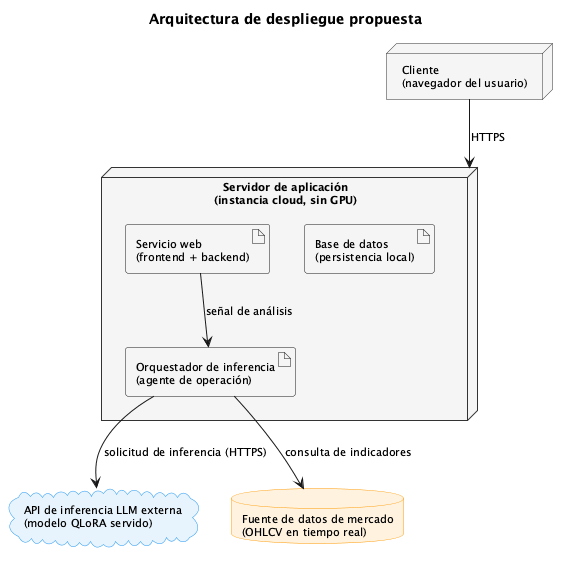
\includegraphics[width=0.8\textwidth]{figures/fig_lightsail.png}
\caption{Arquitectura de despliegue propuesta: servidor de aplicaci\'on sin GPU que delega la inferencia a una API de LLM externa. La separaci\'on entre c\'omputo general e inferencia permite escalar cada componente de forma independiente.}
\label{fig:lightsail}
\end{figure*}

% ── Referencias ──────────────────────────────────────────────────────────────
\footnotesize
\begin{thebibliography}{99}

\bibitem{sun2026}
Z.~Sun and G.~Raskutti, ``A theoretical framework for LLM fine-tuning using early stopping for non-random initialization,'' \textit{arXiv preprint arXiv:2602.13942}, 2026.

\bibitem{fu2024}
X.~Fu, M.~Hirano, and K.~Imajo, ``Financial fine-tuning a large time series model,'' \textit{arXiv preprint arXiv:2412.09880}, 2024.

\bibitem{liu2026}
B.~Liu and R.~Dang, ``FinPos: A position-aware trading agent system for real financial markets,'' \textit{arXiv preprint arXiv:2510.27251}, 2026.

\bibitem{bysik2026}
N.~Bysik and R.~\'Slepaczuk, ``XGBoost and LSTM Models for Bitcoin Price Prediction,'' \textit{arXiv preprint arXiv:2606.00060}, 2026.

\bibitem{miguelanez2026}
C.~Miguela\~nez, ``Fine-tuning LLMs: Hyperparameter best practices,'' \textit{Latitude.so}, Feb.~2, 2026.

\bibitem{mitrasish2026}
Mitrasish, ``How to fine-tune LLMs in 2026: Costs, GPUs, and code,'' \textit{Spheron Blog}, Mar.~5, 2026.

\bibitem{pan2026}
Y.~Pan and S.~C.~Liew, ``Learning to trade like an expert: Cognitive fine-tuning for stable financial reasoning in language models,'' \textit{arXiv preprint arXiv:2604.16862}, 2026.

\bibitem{unsloth2026}
Unsloth, ``LoRA fine-tuning hyperparameters guide,'' \textit{Unsloth Documentation}, 2026.

\bibitem{dettmers2023}
T.~Dettmers \textit{et al.}, ``QLoRA: Efficient Finetuning of Quantized Language Models,'' in \textit{Proc. NeurIPS}, 2023.

\bibitem{hu2021}
E.~Hu \textit{et al.}, ``LoRA: Low-Rank Adaptation of Large Language Models,'' in \textit{Proc. ICLR}, 2022.

\bibitem{nimmaturi2025}
D.~Nimmaturi \textit{et al.}, ``Predictive scaling laws for efficient GRPO training of large reasoning models,'' \textit{arXiv preprint arXiv:2507.18014}, 2025.

\bibitem{nguyen2026}
P.~Nguyen and T.~Pham, ``Toward reliable evaluation of LLM-based financial multi-agent systems: Taxonomy, coordination primacy, and cost awareness,'' \textit{arXiv preprint arXiv:2603.27539}, 2026.

\bibitem{ruan2025}
Z.~Ruan \textit{et al.}, ``Unveiling over-memorization in finetuning LLMs for reasoning tasks,'' \textit{arXiv preprint arXiv:2508.04117}, 2025.

\bibitem{lopez2023}
A.~Lopez-Lira and Y.~Tang, ``Can ChatGPT Forecast Stock Price Movements?'' \textit{arXiv preprint arXiv:2304.07619}, 2023.

\bibitem{pindza2026}
E.~Pindza, ``Testing ML trading strategies with purged walk-forward validation,'' \textit{Frontiers in Blockchain}, 2026.

\bibitem{mcnemar1947}
Q.~McNemar, ``Note on the sampling error of the difference between correlated proportions,'' \textit{Psychometrika}, vol.~12, no.~2, pp.~153--157, 1947.

\bibitem{pardo2008}
R.~Pardo, \textit{The Evaluation and Optimization of Trading Strategies}, 2nd~ed. Wiley, 2008.

\bibitem{qwen2024}
Qwen Team, ``Qwen2.5 Technical Report,'' Alibaba Cloud, 2024. [Online]. Available: \url{https://qwenlm.github.io/blog/qwen2.5/}

\bibitem{bouri2017}
E.~Bouri, P.~Molnar, G.~Azzi, D.~Roubaud, and L.~I.~Hagfors, ``On the hedge and safe haven properties of Bitcoin: Is it really more than a diversifier?'' \textit{Finance Research Letters}, vol.~20, pp.~192--198, 2017.

\bibitem{repo}
A.~Gonz\'alez~Almaz\'an, ``Trading Management --- Repositorio del proyecto,'' 2026. [Online]. Available: \url{https://github.com/alejandrogonzalz/trading_management}

\end{thebibliography}

\end{document}
